\chapter{3D目标检测与位姿估计算法}
\label{chap:pose}
本章介绍了本文所设计的基于RGB-D图像的3D目标检测和位姿估计算法3D-MRAI(3D Mask R-CNN with Angle-fixed-4PCS and ICP),该算法根据所提供目标的CAD模型,可以在RGB-D图中检测出目标,并给出目标的位姿。所提出的3D-MRAI算法主要有两个模块构成:检测模块和匹配模块。检测模块基于Mask R-CNN\cite{He2017}实现在3D点云中定位目标,匹配模块通过匹配目标3D模型和由检测模块定位的目标点云实现对目标的位姿估计。为了评价所设计的3D-MRAI算法的性能,本章还设计了相关实验,并与同类算法相比较,从算法的检测准确度、位姿精度和时间性能三个方面分析了算法性能。

\section{3D-MRAI框架设计}
本文设计的3D-MRAI算法主要解决三维空间中的目标检测和位姿估计问题,根据输入的RGB-D图像,输出图像中的目标和其在三维空间中的位姿,区别于常见的2D目标检测算法(2D目标检测算法往往只给出目标的种类和其在图像坐标中的Bounding box或者Mask)。给出目标在三维空间中的位姿的意义十分巨大,尤其在机器人领域中,图像层面的结果往往难以满足要求,但同时算法的难度也很大。

一些给出3D目标位姿的传统算法,如3DMatch\cite{zeng20163dmatch},3DMatch通过匹配局部几何特征来计算目标的位姿,缺点是对采集的3D数据质量要求很高,往往需要使用激光采集,因此整个识别过程的时间很久;通过SIFT描述子来匹配目标位姿\cite{dias2015sift}也是一种方法,但其对纹理较少的物体往往难以匹配,效果很差;另外如LINEMOD\cite{hinterstoisser2012gradient}和MOPED\cite{collet2011moped}这些位姿估计框架,在某些情况下如目标在平整的桌面上并且光照条件较好的情况下才能取得满意的效果。因此,传统的一些3D目标位姿估计算法往往难以在实际中具体应用,为此,本文设计一种鲁棒性和准确率都较高的3D目标检测和位姿估计算法3D-MRAI。

所设计的3D-MRAI算法的框架如图\ref{fig:detect-pose}所示,
\begin{figure}[ht]
  \centering
  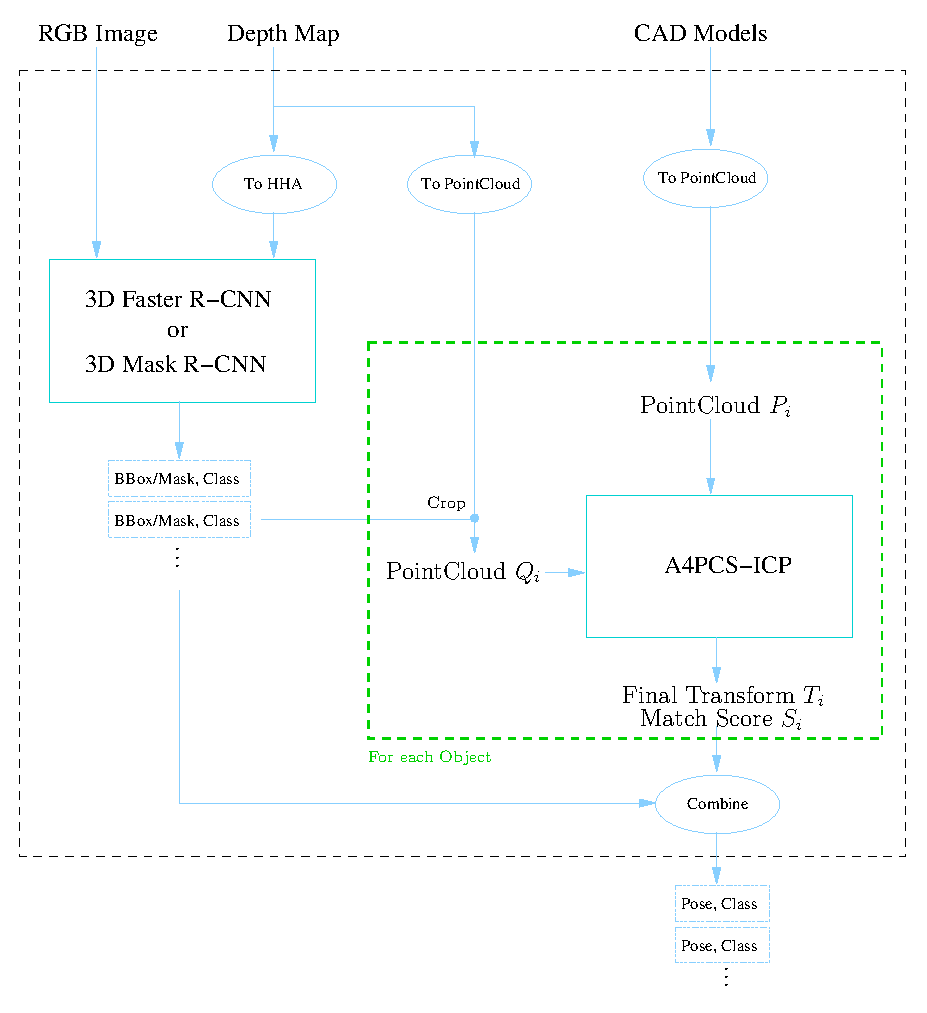
\includegraphics[width=12cm]{detect-pose}
  \caption{3D-MRAI算法框架}
  \label{fig:detect-pose}
\end{figure}
从图\ref{fig:detect-pose}可以看出算法的输入是RGB图像、深度图,以及目标物体的CAD模型,输出是图像中检测到的目标的位姿。所设计的3D-MRAI算法的核心部分为两个模块:检测模块和匹配模块。检测模块通过引入HHA(Horizontal disparity, Height above ground, Angle with gravity)和STN(Spatial Transformer Network)将Faster R-CNN\cite{Ren}和Mask R-CNN\cite{He2017}扩展到RGB-D图像上来,使其检测缺少纹理目标的准确率大大提升;匹配模块在4PCS算法\cite{aiger20084}的基础上,对其进行改进,减少了算法运算时间,并通过ICP算法\cite{besl1992method}迭代提高匹配精度。两个模块完成的主要功能如下:
\begin{itemize}
\item {\kai 检测模块}:在RGB-D图中检测出目标,得到目标BBox(Bounding Box)或者Mask
\item {\kai 匹配模块}:将目标3D模型与由BBox/Mask分割的目标点云进行匹配,得到目标位姿
\end{itemize}

\section{检测模块}
\label{sec:detector}
\subsection{模块框架设计}
本文所设计的检测模块有两种:一种基于Faster R-CNN,另外一种基于Mask R-CNN。两种模块的输出不同,基于Faster R-CNN的检测模块在RGB-D图中输出的是目标的Class和BBox;基于Mask R-CNN的检测模块输出的是目标的Class、BBox和Mask。从模块输出来看,基于Faster R-CNN的检测模块是基于Mask R-CNN的检测模块的子集。在设计之初,基于Faster R-CNN的检测模块先被设计出来,由于基于Faster R-CNN的检测模块的输出只有Class和BBox,对于普通物体通过BBox分割目标点云再输入到匹配模块进行匹配并没有什么问题,但是,当所要检测的物体是细长类型的,在某些位姿下,如图\ref{fig:bbox-segment}所示BBox内的大部分像素都不是目标物体,此时通过该BBox分割得到的目标点云也包含了许多不属于该目标的点,这样的点云输入到匹配模块很难进行正确的匹配。
\begin{figure}[ht]
  \centering
  \subfloat[检测模块输出的BBox示意图]{
    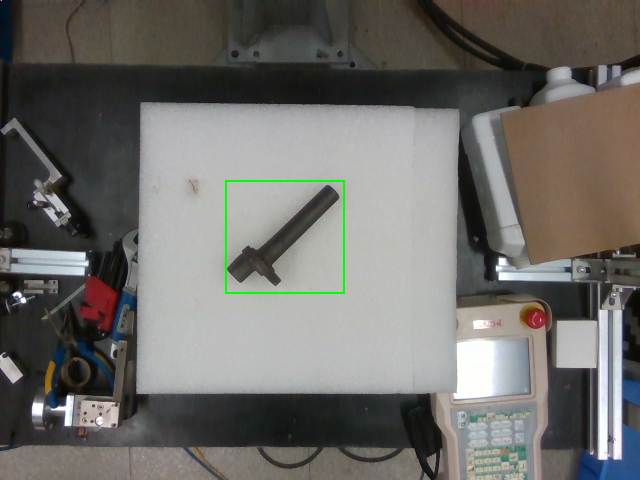
\includegraphics[width=6cm]{bbox-segment}
  }
  \hskip1cm
  \subfloat[根据BBox分割得到的点云]{
    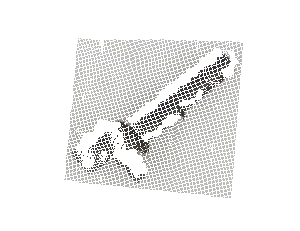
\includegraphics[width=6cm]{bbox-segment-cloud}
  }
  \caption{由BBox分割点云效果图}
  \label{fig:bbox-segment}
\end{figure}

\begin{figure}[ht]
  \centering
  \subfloat[检测模块输出的Mask示意图]{
    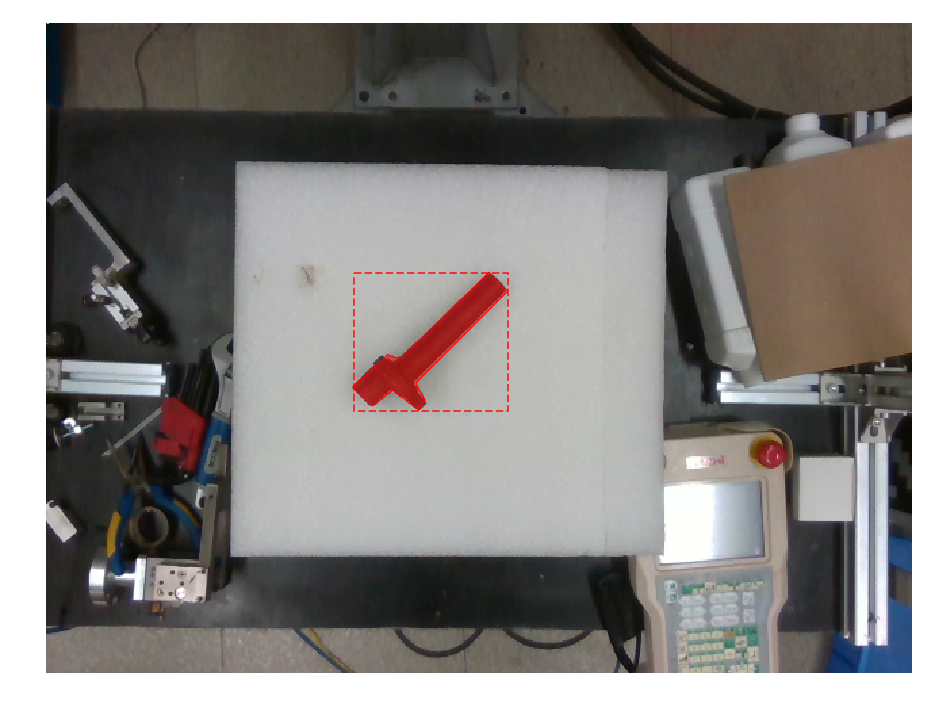
\includegraphics[width=6cm]{mask-segment}
  }
  \hskip1cm
  \subfloat[根据Mask分割得到的点云]{
    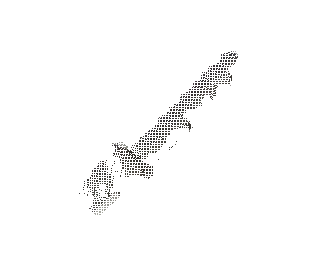
\includegraphics[width=6cm]{mask-segment-cloud}
  }
  \caption{由Mask分割点云效果图}
  \label{fig:mask-segment}
\end{figure}
为了解决这一个问题,本文参考Mask R-CNN对Faster R-CNN的改进,设计了基于Mask R-CNN的检测模块,通过Mask R-CNN检测输出的Mask分割点云,有效的解决了利用BBox分割细长物体时造成目标点云包含过多不属于目标的点的问题,如图\ref{fig:mask-segment}所示。但是,基于Faster R-CNN的检测模块也有其存在的必要,因为基于Mask R-CNN的检测模块的运算时间要大于基于Faster R-CNN的检测模块,所以,如果考虑算法的时间性能,对于细长物体建议使用基于Mask R-CNN的检测模块,除此之外使用基于Faster R-CNN的检测模块。

基于Faster R-CNN的检测模块的框架如图\ref{fig:3d_faster_rcnn}所示,基于Mask R-CNN的检测模块的框架如图\ref{fig:3d_mask_rcnn}所示。
\begin{figure}[ht]
  \centering
  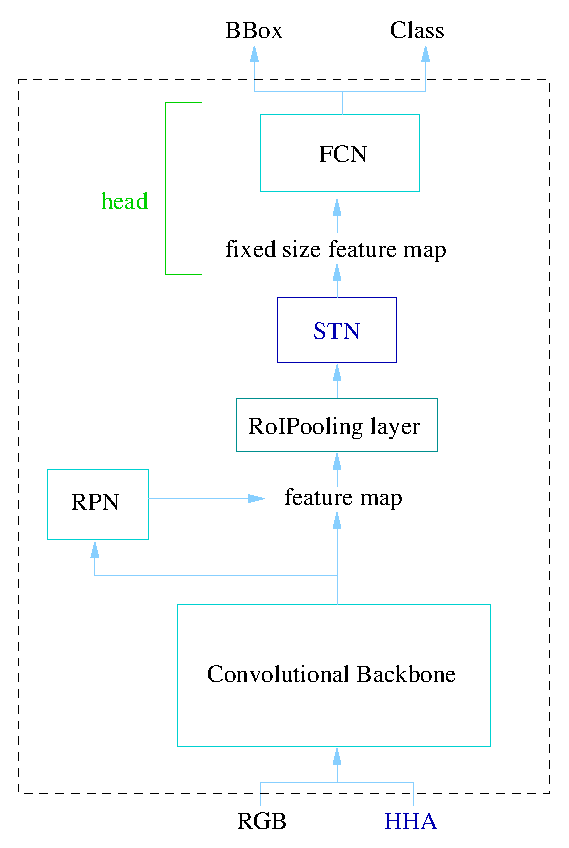
\includegraphics[width=8cm]{faster_rcnn_module}
  \caption{基于Faster R-CNN的检测模块}
  \label{fig:3d_faster_rcnn}
\end{figure}
\begin{figure}[ht]
  \centering
  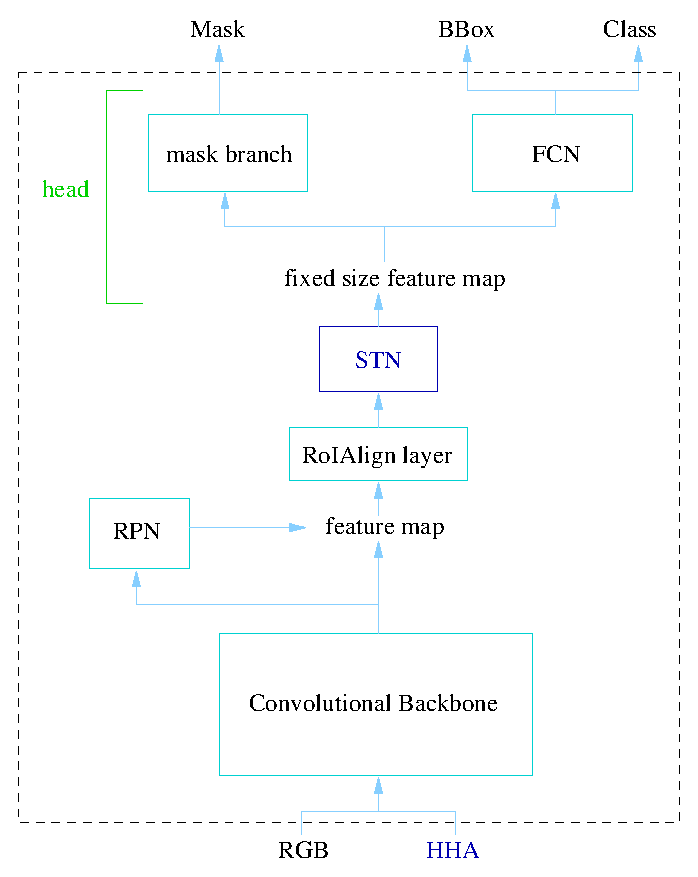
\includegraphics[width=10cm]{mask_rcnn_module}
  \caption{基于Mask R-CNN的检测模块}
  \label{fig:3d_mask_rcnn}
\end{figure}
两个检测模块对Faster R-CNN和Mask R-CNN的改进相同,因此本文主要介绍对Mask R-CNN的改进,对Faster R-CNN的改进类似。

\subsection{对Mask R-CNN的改进}
Mask R-CNN是一个2D目标检测的深度神经网络,其网络结构如图\ref{fig:mask_rcnn}所示。
\begin{figure}[ht]
  \centering
  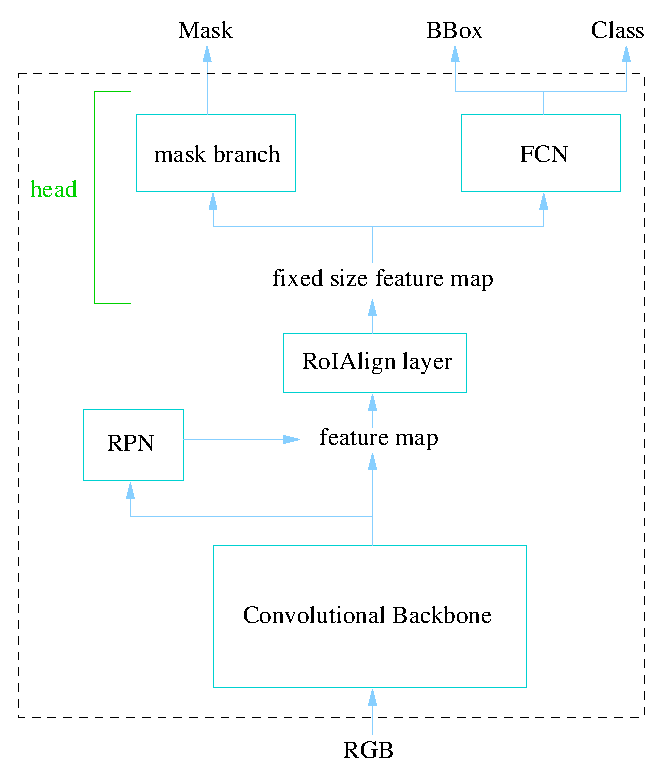
\includegraphics[width=10cm]{mask_rcnn}
  \caption{Mask R-CNN网络结构}
  \label{fig:mask_rcnn}
\end{figure}
Mask R-CNN在Faster R-CNN的基础上通过增加一个Mask分支,使得网络不仅可以输出目标的Class和BBox,还可以输出目标的Mask。除此之外,Mask R-CNN还通过改用ResNeXt-101+FPN强化了Faster R-CNN中的特征提取网络(convolutional backbone),其中ResNeXt\cite{xie2017aggregated}是残查网络ResNet\cite{he2016deep}的改进, ResNeXt结构可以在不增加参数复杂度的前提下提高准确率,同时还减少了超参数的数量;FPN(Feature Pyramid Networks)\cite{lin2017feature}利用了深度卷积神经网络固有的多尺度、多层级的金字塔结构去构建特征金字塔网络来提升检测的准确度。Mask R-CNN还提出了ROIAlign层,替换掉Faster R-CNN中的ROIPooling层,从而解决ROIPooling造成的像素不对齐问题,实现预测Pixel级别的Mask。

本文所设计的检测模块对Mask R-CNN的改进主要有两点:
\begin{itemize}
\item 将深度图转化为HHA图与RGB图一起输入到网络
\item 在ROIAlign层后面增加了STN
\end{itemize}

Mask R-CNN网络本来的输入是RGB图,经过实验测试,本文发现单单通过RGB图Mask R-CNN难以检测一堆缺少纹理的物体(Textureless Object)。对于缺少纹理的物体虽然在RGB图中难以检测,但是其在深度图中信息还没有有效利用,所以可以尝试将RGB图和深度图相结合。

从2012年AlexNet\cite{Krizhevsky2012}在ImageNet\cite{imagenet}数据集上的应用开始,深度学习在彩色图上的应用已经相当成熟,但深度学习在深度图上的应用还比较少,如何使用CNN在深度图上提取特征是一个值得探讨的问题,是将深度图直接作为一个通道使用CNN提取特征?还是将深度图变换到三维坐标(x,y,z),然后再在这三个通道上通过CNN提取特征?经过实验和相关调研,本文发现将深度图转换为HHA图后进行训练的模型有较高的准确率\cite{Gupta2014},因此本文将深度图转换为HHA三个通道,然后再通过CNN提取特征。HHA三个通道的分别为:
\begin{itemize}
\item 水平方向上视差(Horizontal disparity)
\item 距离地面的高度(Height above ground)
\item 法向量与重力的夹角(Angle with gravity)
\end{itemize}

\emph{Horizontal disparity}:深度图到视差的转换相对来说十分简单,理论上视差与深度呈倒数关系,因此水平方向上的视差计算具体如算法\ref{alg:hd}所示。
\begin{algorithm}[!ht]
  \caption{计算水平方向上视差}
  \label{alg:hd}
  \KwIn{Depth Frame $D_{h\times w}$}
  \KwOut{Horizontal disparity Frame $H_{h\times w}$}
  $h_{floor} = 1 / d_{ceil}, h_{ceil} = 1 / d_{floor}$\;
  \For {$y\leftarrow 1$ \KwTo $h$} {
    \For {$x\leftarrow 1$ \KwTo $w$} {
      $H[y, x] = 1 / D[y, x]$\;
      $H[y, x] = (H[y, x] - h_{floor}) / (h_{ceil} - h_{floor})$\;
    }
  }
\end{algorithm}

\emph{Height above ground}:计算距离地面的高度首先要确定一个世界坐标系,然后得到世界坐标系到相机坐标系的旋转矩阵$\prescript{W}{C}{R}$和平移向量$\prescript{W}{C}{T}$,最后通过坐标变换得到距离地面的高度,具体如算法\ref{alg:hg}所示。
\begin{algorithm}[!ht]
  \caption{计算距离地面的高度}
  \label{alg:hg}
  \KwIn{Point Cloud $P_{h\times w}$}
  \KwOut{Hight Frame $H_{h\times w}$}
  \For {$y\leftarrow 1$ \KwTo $h$} {
    \For {$x\leftarrow 1$ \KwTo $w$} {
      $p =  \prescript{W}{C}{R}P[y, x] + \prescript{W}{C}{T}$\;
      $H[y, x] = p.z$\;
    }
  }
\end{algorithm}

\emph{Angle with gravity}:法向量与重力的夹角的计算相对来说稍微复杂一点,重力的方向在工作区间内一般与所设的世界坐标系的$z$轴负方向相同,因此原问题就是求法向量与世界坐标系$z$轴负方向之间的夹角。参考文献\cite{Gupta2013},首先计算深度图中每个点上的法向量,计算点云中一点$p_0$的法向量$\vec{n}$的简单思路如下:
\begin{itemize}
\item 找出距离点$p_0$最近的$k$个点:$p_1, p_2,...p_k$
\item 通过最小二乘在点$\{p_i|i = 0, 1, \ldots , k\}$中拟合出平面$Ax + By + Cz + D = 0$
\item 点$p_0$的法向量$\vec{n} = [A, B, C]^T$
\end{itemize}
考虑到所采集的深度图转换的点云是有序的(Organized Point Cloud),意味着坐标索引相近的点实际物理距离也相近,因此找出距离点$p_0$最近的$k$个点可以通过选取点$p_0$坐标索引附近的点代替,具体地,记点$p_0$在深度图中图像坐标为$(x_0, y_0)$,取点集$\bm{S} = \{p_i|x_0 - R \leq x_i \leq x_0 + R , y_0 -R \leq y_i \leq y_0 + R\}$,其中$R$是选取区域的半径。得到法向量后计算法向量与世界坐标$z$轴负方向的角度就十分简单了,整个计算法向量与重力的夹角的算法如\ref{alg:angle}所示。
\begin{algorithm}[!ht]
  \caption{计算法向量与重力的夹角}
  \label{alg:angle}
  \KwIn{Point Cloud $P_{h\times w}$}
  \KwOut{Angle Frame $A_{h\times w}$}
  \For {$y\leftarrow 1$ \KwTo $h$} {
    \For {$x\leftarrow 1$ \KwTo $w$} {
      Calculate surface normal $\prescript{C}{}{\vec{n}}$ at point $P[y,x]$\;
      $\prescript{W}{}{\vec{n}} =  \prescript{W}{C}{R}\prescript{C}{}{\vec{n}} + \prescript{W}{C}{T}$\;
      $A[y, x] = arccos(-(\vec{n}\cdot\vec{oz}) / (|\vec{n}||\vec{oz}|))$\;
    }
  }
\end{algorithm}

计算完上述HHA三个通道后,为了计算和存储方便,分别将三个通道的值线性变换到0到255之间,可视化如图\ref{fig:hha}所示。
\begin{figure}
  \centering
  \subfloat[深度图]{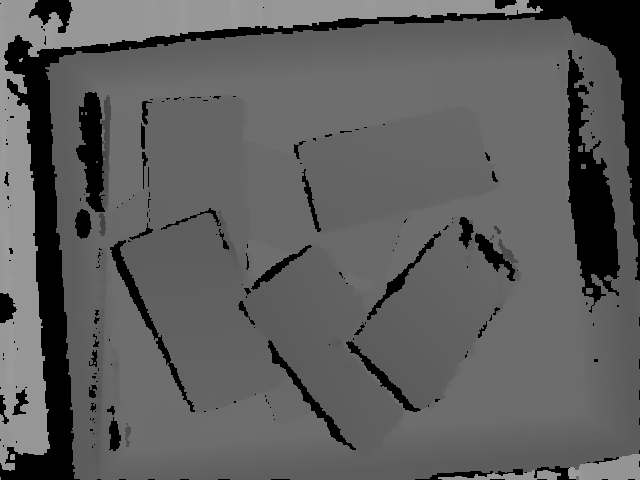
\includegraphics[width=4.5cm]{depth_frame}}
  \hskip5em
  \subfloat[HHA图]{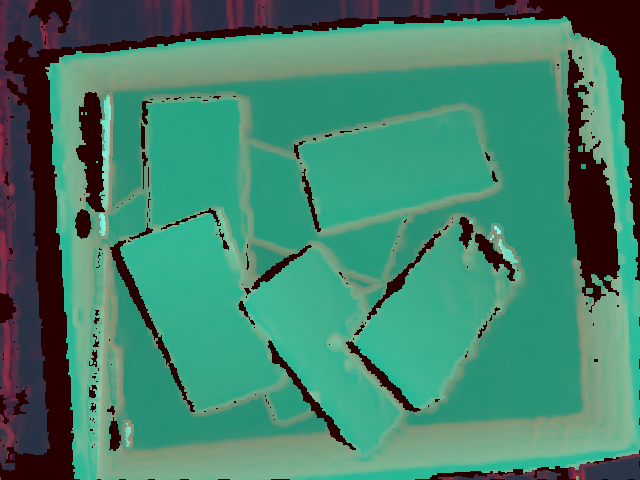
\includegraphics[width=4.5cm]{hha_frame}}
  \vfill
  \subfloat[水平视差图]{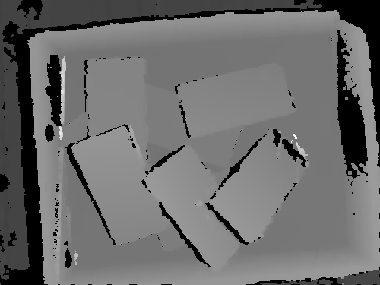
\includegraphics[width=4.5cm]{disparity_frame}}
  \hfill
  \subfloat[距离地面高度图]{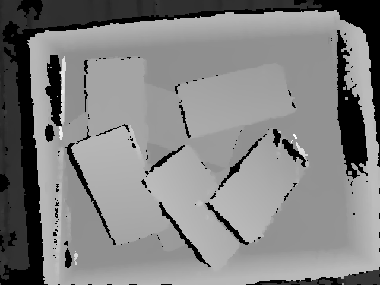
\includegraphics[width=4.5cm]{height_frame}}
  \hfill
  \subfloat[法向量与重力夹角图]{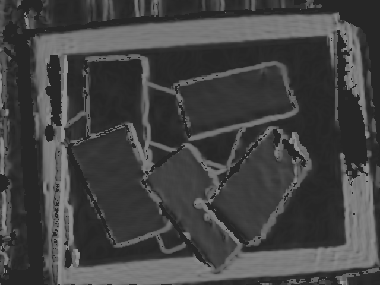
\includegraphics[width=4.5cm]{angle_frame}}
  \caption{HHA可视化效果图}
  \label{fig:hha}
\end{figure}

Mask R-CNN除了难以检测一堆缺少纹理的物体外,本文还发现Mask R-CNN训练得到的模型对物体旋转较为敏感,如图\ref{fig:cat}所示,
\begin{figure}[!ht]
  \centering
  \subfloat[检测旋转前的图片\label{fig:rotation1}]{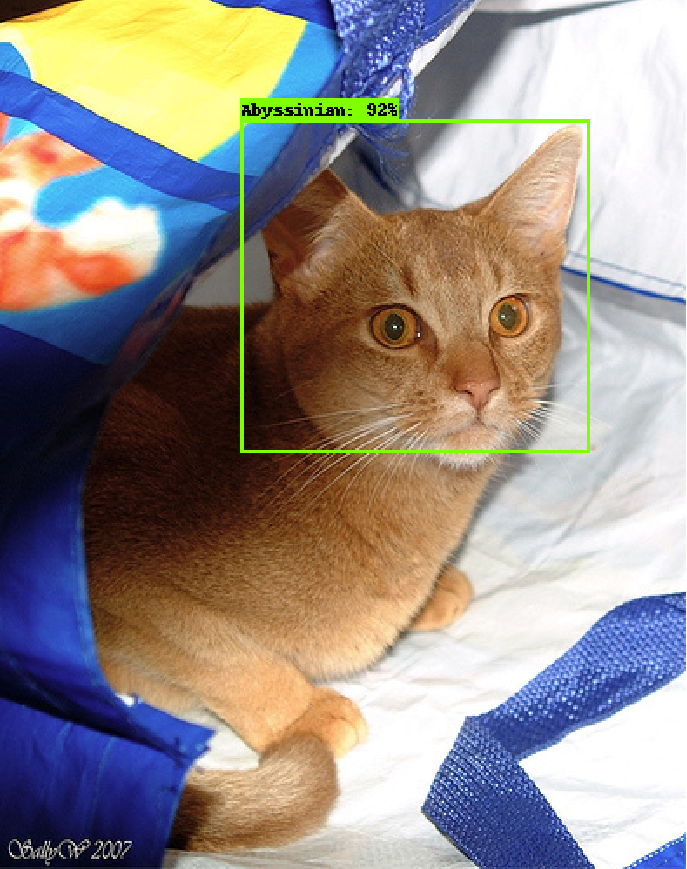
\includegraphics[width=4cm]{cat_up}}
  \hskip1em
  \subfloat[检测旋转后的图片\label{fig:rotation2}]{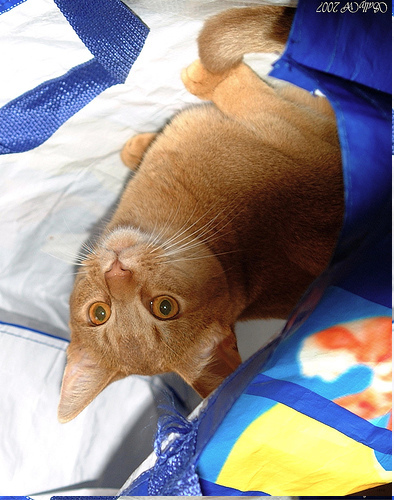
\includegraphics[width=4cm]{cat_down}}
  \caption{检测模型对旋转敏感}
  \label{fig:cat}
\end{figure}
其中图\ref{fig:rotation2}只是将图\ref{fig:rotation1}旋转了180度,由于CNN所提取的特征不具有旋转不变性,并且训练集中的图片宠物都是头朝上的,即使图\ref{fig:rotation1}在训练集中,将其旋转180度后,也无法从中检测出目标来。解决这个问题有两个思路:
\begin{itemize}
\item Data Augmentation
\item Spatial Transformer Network
\end{itemize}
Data Augmentation是通过对训练集中的图片进行旋转以获取不同角度的图片,通过这种方式增大数据集从而使得最终训练得到的模型对各种角度的图片都能识别;Spatial Transformer Network是一种特殊的网络结构,本文所使用的就这种方式。

Spatial Transformer Network是一个可微模块,根据输入的特征对其进行相应的空间变化,输出变换后的特征,如图\ref{fig:spatial_transformer_results}所示,
\begin{figure}[ht]
  \centering
  \subfloat{
    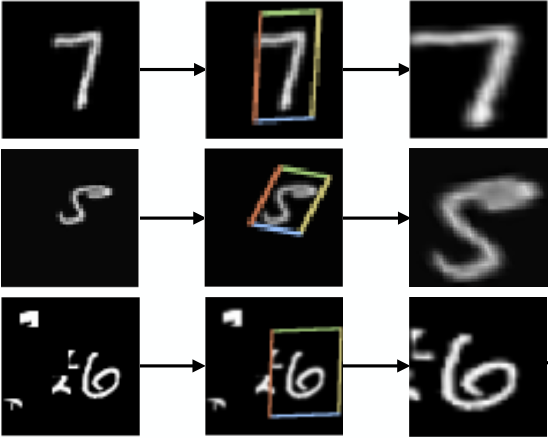
\includegraphics[width=6cm]{stn_results}
  }
  \hskip0.5cm
  \subfloat{
    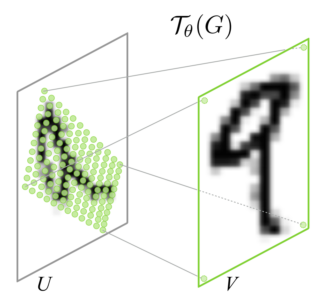
\includegraphics[width=6cm]{grid-generator}
  }
  \caption{Spatial Transformer Network效果图}
  \label{fig:spatial_transformer_results}
\end{figure}
输入特征$U$经过Spatial Transformer Network模块后输出特征$V$。Spatial Transformer Network模块具体可以分为三个部分,如图\ref{fig:spatial_transformer}。
\begin{figure}[ht]
  \centering
  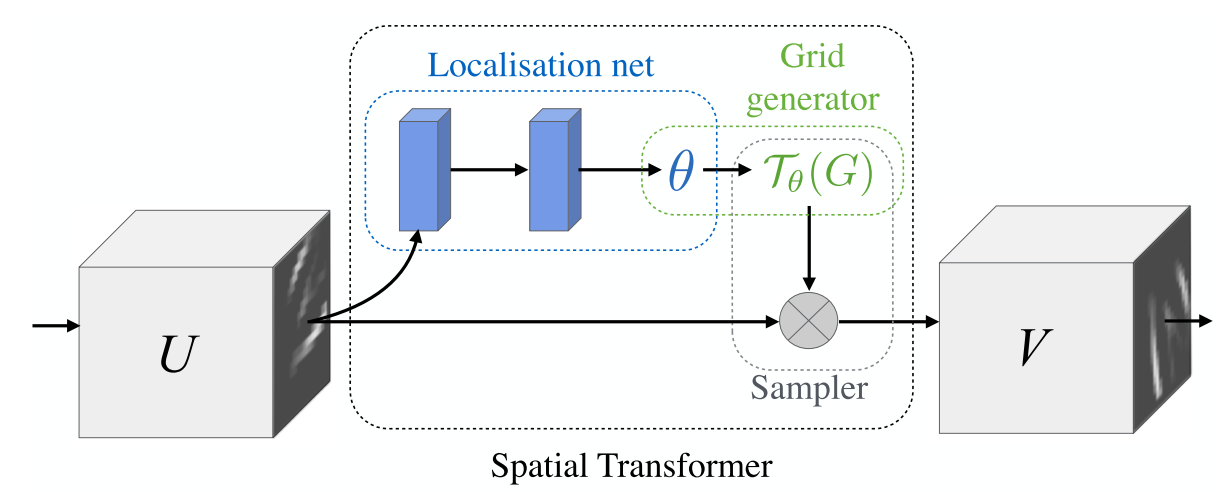
\includegraphics[width=12cm]{stn_structure}
  \caption{Spatial Transformer Network结构图}
  \label{fig:spatial_transformer}
\end{figure}
简单来讲,第一部分是一个定位网络(localisation network),输入特征$U$,输出需要进行空间变换的参数;第二部分是一个网格生成器(grid generator),根据空间变换的参数生成输入特征中需要变换的点的网格;第三部分是个采样器,根据网格生成器的输出对输入特征进行采样并进行空间变换,生成输出特征。

具体地,记定位网络的输入为特征$U\in \mathbb{R}^{H\times W\times C}$,其中$W,H,C$分别为长、宽和通道数,网络的输出为空间变化$\mathcal{T}_{\theta}$的参数$\theta$,参数$\theta$的个数由空间变换的类型决定,本文所采用的空间变换为2D仿射变换,则
\begin{equation}
  \mathcal{T}_\theta = \left[
    \begin{array}{ccc}
      \theta_{11}&\theta_{12}&\theta_{13}\\
      \theta_{21}&\theta_{22}&\theta_{23}
    \end{array}
    \right]
\end{equation}
定位网络内部可以由一些全连接层或者卷积层再加一个回归层组成。

网格生成器本质上就是在输入特征中选取需要进行空间变化的点,如图\ref{fig:spatial_transformer_results}中绿色点便是网格生成器所选取的点,记Spatial Transformer Network的输出特征为$V\in \mathbb{R}^{H'\times W'\times C}$,其中$W',H',C$分别为输出特征的长、宽和通道数,输出特征的通道数和输入特征的通道数相同,不能改变,并且空间变换$\mathcal{T}_{\theta}$将分别作用于输入$U$的各个通道以保证每个通道上的变换一致。并记点集$G = \{G_i|G_i = (x^t_i, y^t_i)\}$,其中$(x_i^s, y_i^s)$为输出特征图中点的坐标,由定位网络输出的参数$\theta$和$G$我们就可以在输入特征中确定需要进行空间变换的点的集合$\mathcal{T}_\theta(G)$:
\begin{equation}
  \left(
    \begin{array}{c}
      x_i^s\\
      y_i^s
    \end{array}
  \right) = \mathcal{T}_\theta(G_i) =
  \left[
    \begin{array}{ccc}
    \theta_{11}&\theta_{12}&\theta_{13}\\
    \theta_{21}&\theta_{22}&\theta_{23}
    \end{array}
  \right]
  \left(
    \begin{array}{c}
      x_i^t\\
      y_i^t\\
      1\\
    \end{array}
  \right)
\end{equation}
其中$(x_i^s, y_i^s)$是输入特征中点的坐标,也是图\ref{fig:spatial_transformer_results}中的绿色点。

采样器输入网格生成器生成的点集$\mathcal{T}_\theta$,和输入特征$U$,最终输出经过空间变换后的特征$V$,具体如公式\ref{eq:sampler}所示:
\begin{equation}
  \label{eq:sampler}
  V_i^c = \sum_n^H\sum_m^W{U_{nm}^ck(x_i^s-m;\Phi_x)k(y_i^s-n;\Phi_y)}\quad \forall i\in[1\ldots H'W']\quad \forall c\in[1\ldots C]
\end{equation}
其中$\Phi_{x}$和$\Phi_{y}$是采样核函数$k()$的参数,$U_{nm}^c$表示输入特征$U$在坐标$(n, m)$下第$c$个通道上的值,$V_i^c$表示输出特征在坐标$(x_i^t,y_i^t)$下第$c$个通道上的值。理论上可以使用任何采样核函数,只要可以对$x_i^s$和$y_i^s$求导,因为网络训练需要对公式\ref{eq:sampler}求导。以双线性采样核函数为例,公式\ref{eq:sampler}变为
\begin{equation}
  V_i^c = \sum_n^H\sum_m^W{U_{nm}^cmax(0, 1-|x_i^s-m|)max(0, 1-|y_i^s-n|)}
\end{equation}
则$V$对$U$和$G$的梯度为
\begin{equation}
  \frac{\partial V_i^c}{\partial U_{nm}^c} = \sum_n^H\sum_m^W{max(0, 1-|x_i^s-m|)max(0, 1-|y_i^s-n|)}
\end{equation}
\begin{equation}
  \frac{\partial V_i^c}{\partial x_i^s} = \sum_n^H\sum_m^W{U_{nm}^cmax(0, 1-|y_i^s-n|)}
  \left\{
      \begin{array}{ll}
        0&if\; |m-x_i^s| \geq 1\\
        1&if\; m \geq x_i^s\\
        -1&if\; m < x_i^s
      \end{array}
    \right.
\end{equation}
\begin{equation}
  \frac{\partial V_i^c}{\partial y_i^s} = \sum_n^H\sum_m^W{U_{nm}^cmax(0, 1-|x_i^s-m|)}
  \left\{
      \begin{array}{ll}
        0&if\; |n-y_i^s| \geq 1\\
        1&if\; n \geq y_i^s\\
        -1&if\; n < y_i^s
      \end{array}
    \right.
\end{equation}

具体地,对于Mask R-CNN本文将STN模块加在了Mask R-CNN的ROIAlign层之后,如图\ref{fig:mask_rcnn}所示。通过在ROIAlign层后增加STN模块,使得提取的特征经过STN模块后具有一定的旋转不变性。

\subsection{检测模块实验}
为了评价所设计的基于Faster R-CNN和Mask R-CNN的检测模块的性能,本文分别在一个现有的数据集和一个自己采集的实际应用的数据集上进行了网络的训练和测试,并与原始的Faster R-CNN和Mask R-CNN网络相比较,验证了所设计的检测模块的性能。

{\kai 数据集}:实验所采用的数据集一个是参加APC(Amazon Picking Challenge)的MIT-Princeton队伍所采集的数据集"Shelf \& Tote" Benchmark Dataset\cite{apcdataset},此处简单记为APC数据集,另外一个数据集是实际用于Bin-Picking在实验室采集的数据集,记为workpiece数据集。

对于APC数据集,该数据集共有39类不同的物体,452个场景,每个场景有不同的物体,一共7281组图片,通过在多个场景下,不同的视角下使用Intel Realsense SR300相机所拍摄。标注的数据是每个场景下物体在世界坐标系下的位姿,以及每个场景下相机在世界坐标系下的位姿,是一个半自动标注的数据集,通过物体的位姿和相机的位姿就可以得到每个物体在相机坐标系下的位姿,数据集中部分数据如图\ref{fig:apc_dataset}所示。
\begin{figure}[ht]
  \centering
  \subfloat{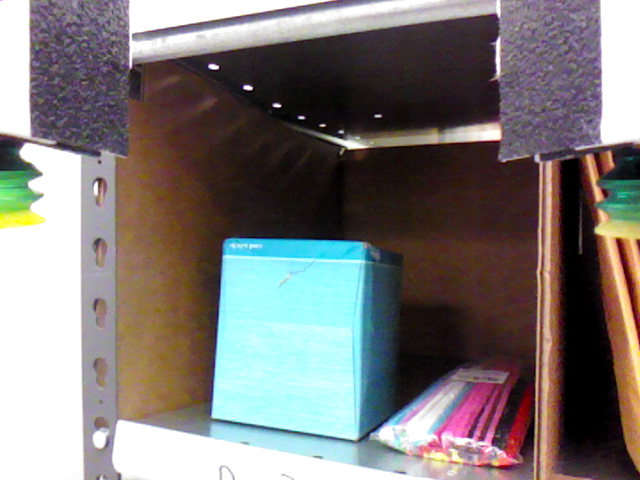
\includegraphics[width=3.5cm]{apc_color1}}
  \hskip0.2cm
  \subfloat{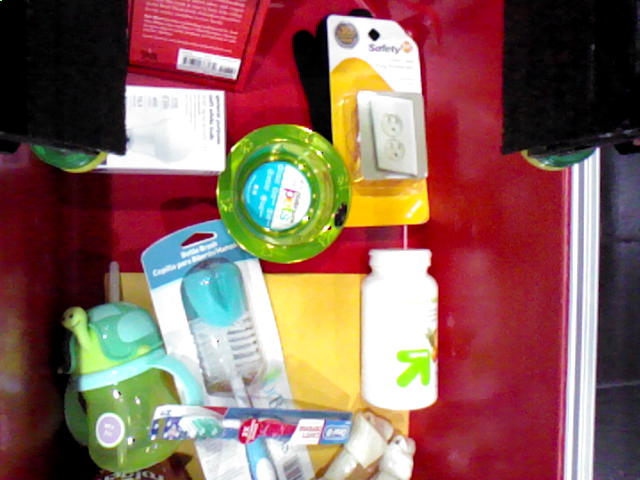
\includegraphics[width=3.5cm]{apc_color2}}
  \hskip0.2cm
  \subfloat{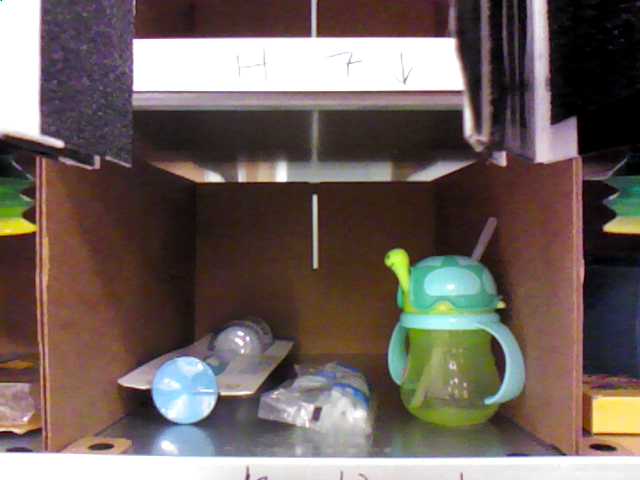
\includegraphics[width=3.5cm]{apc_color3}}
  \hskip0.2cm
  \subfloat{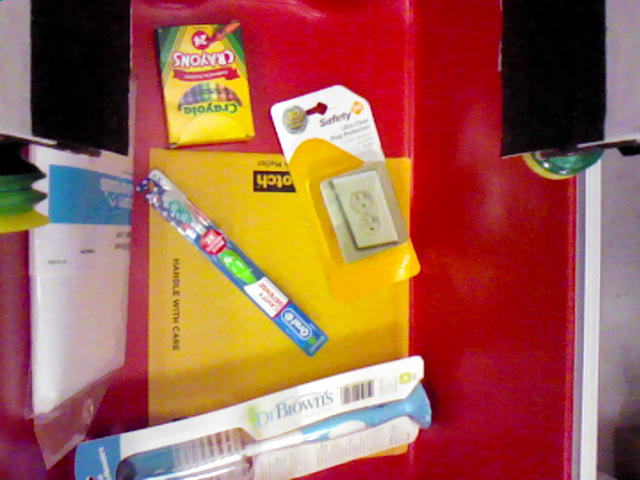
\includegraphics[width=3.5cm]{apc_color4}}
  \vfill
  \subfloat{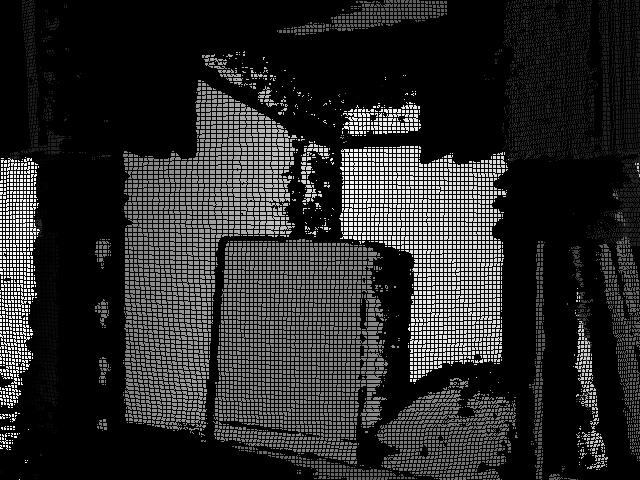
\includegraphics[width=3.5cm]{apc_depth1}}
  \hskip0.2cm
  \subfloat{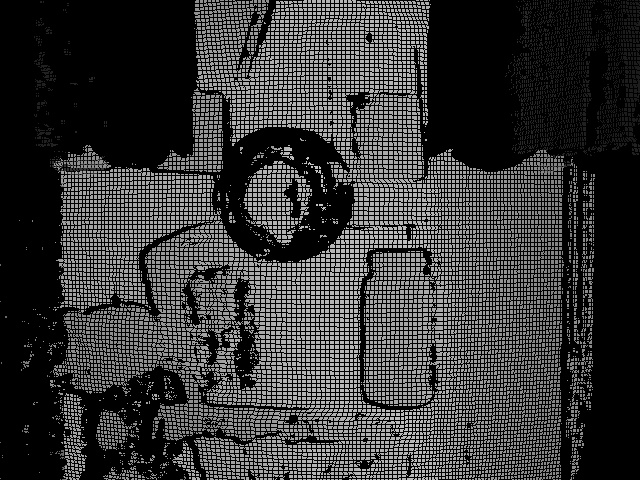
\includegraphics[width=3.5cm]{apc_depth2}}
  \hskip0.2cm
  \subfloat{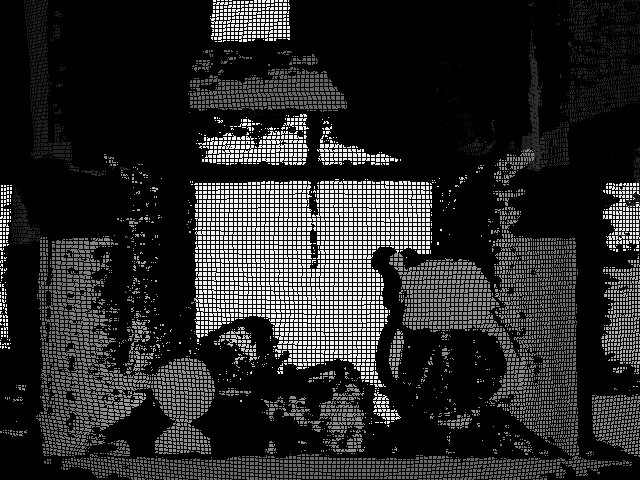
\includegraphics[width=3.5cm]{apc_depth3}}
  \hskip0.2cm
  \subfloat{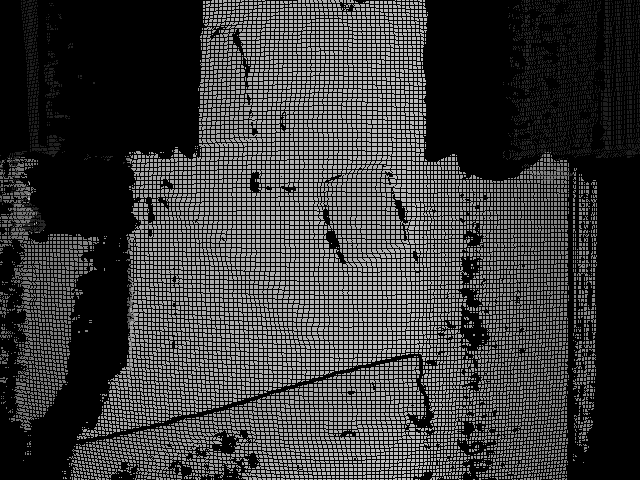
\includegraphics[width=3.5cm]{apc_depth4}}
  \caption{APC数据集部分数据:第一栏为彩色图像,第二栏为与彩色图像相匹配的深度图}
  \label{fig:apc_dataset}
\end{figure}

APC数据集中标注的标签可以认为是每个物体在相机坐标系下的位姿和类别,对于设计的算法来说需要的是物体的类别(Class)、边界框(Bounding Box)和掩模(Mask),因此需要对原始标注数据进行一些处理,因为APC还提供了每类物体的CAD模型,并且相机的内参矩阵也在数据集中提供了,因此可以将CAD模型转换为点云后齐次变换到所标注的对应物体在相机坐标系下的位姿,然后利用相机内参矩阵将物体点云投影到图像平面,从而获得物体的Mask,进而可以得到物体的Bounding Box。需要注意的是由于一个场景中有多个物体,在不同相机位姿下会出现遮挡,因此需要对被遮挡物体的Mask进行相应的裁剪,对于几乎被完全遮挡的物体可以去除掉,判断物体是否遮挡可以通过物体点云距离相机原点的距离远近判断。将一张图中物体位姿得到Mask和Boudning Box的处理流程如下所示:
\begin{enumerate}
\item 对于图中标注的每个物体:
  \begin{itemize}
  \item 将对应物体的3D点云变换到物体标注的位姿
  \item 根据相机内参矩阵将3D点云投影到图像平面,获得物体的Mask以及Mask对应的深度图Depth
  \end{itemize}
\item 遍历像素索引i:
  \begin{itemize}
  \item 如果在索引i出存在多张Mask的值有效,保留Depth值最小的Mask,将其余Mask在索引i处置为无效
  \end{itemize}
\item 对于每个物体的Mask:
  \begin{itemize}
  \item 如果Mask中有效像素点小于阈值$T$,删除该Mask
  \item 根据mask有效像素点的坐标计算对应的Bounding Box
  \end{itemize}
\end{enumerate}
处理后的部分图片的ground truth(Class,Mask,Boudning Box)如图\ref{fig:apc_gt}所示。
\begin{figure}[ht]
  \centering
  \subfloat{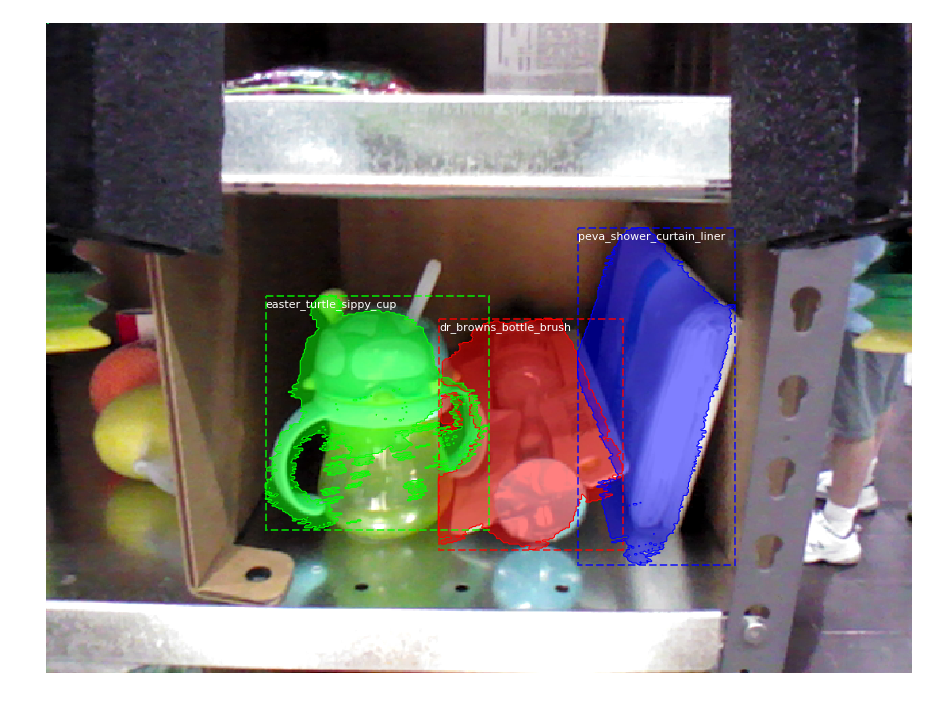
\includegraphics[width=6cm]{apc_gt1}}
  \hskip1cm
  \subfloat{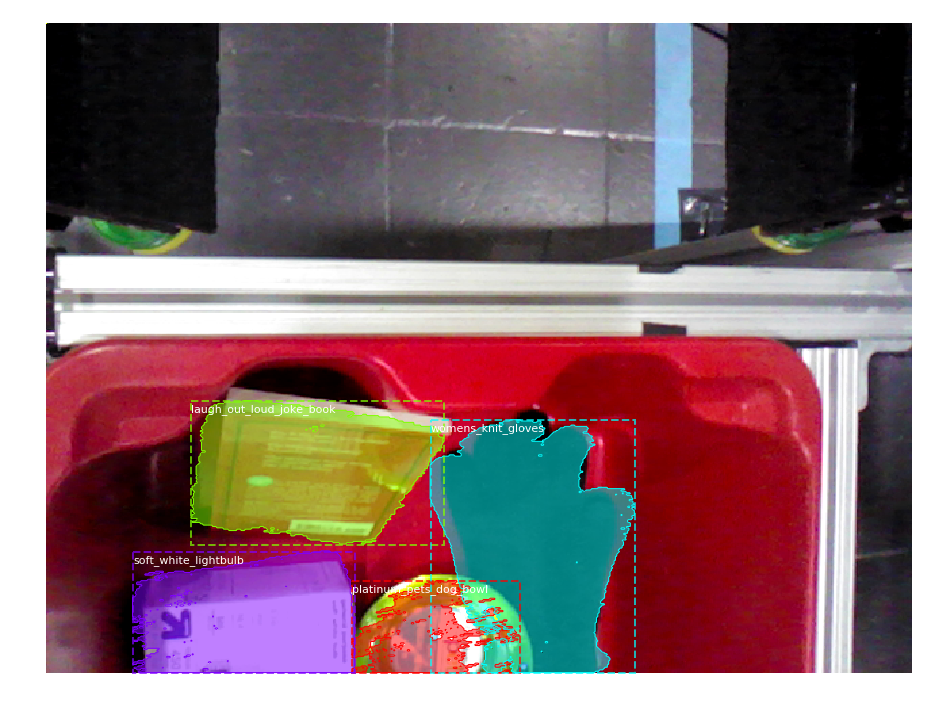
\includegraphics[width=6cm]{apc_gt2}}
  \vfill
  \subfloat{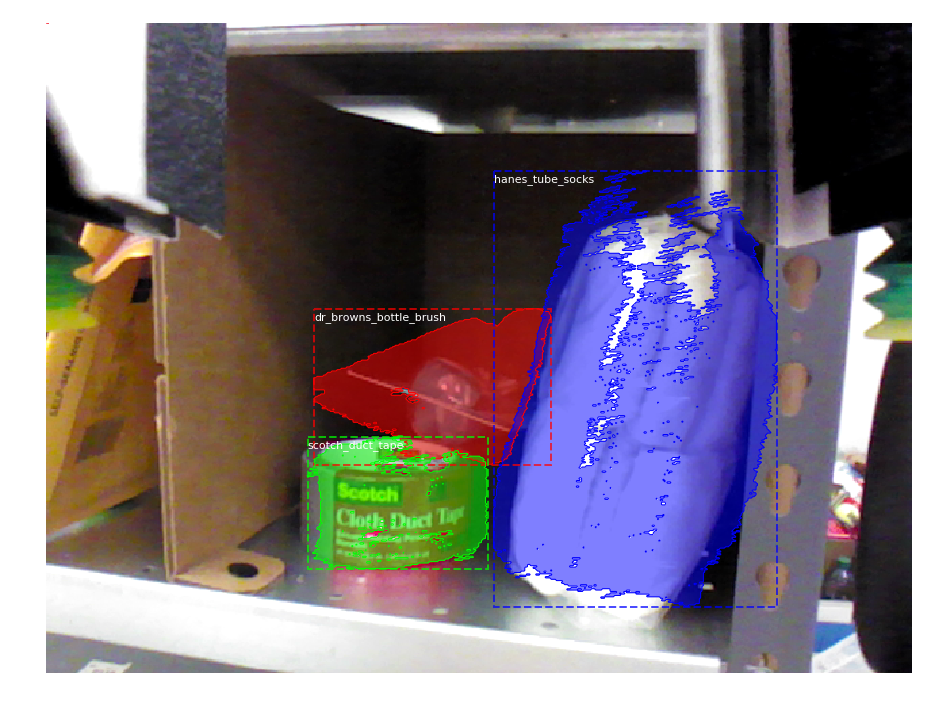
\includegraphics[width=6cm]{apc_gt3}}
  \hskip1cm
  \subfloat{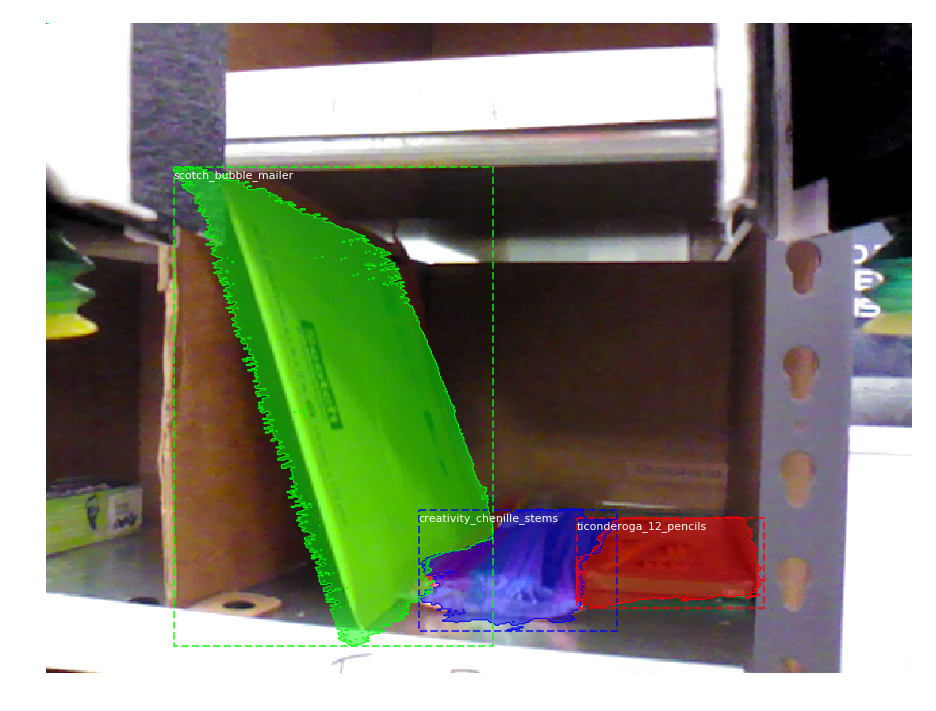
\includegraphics[width=6cm]{apc_gt4}}
  \caption{APC数据集部分标注数据}
  \label{fig:apc_gt}
\end{figure}
从图\ref{fig:apc_gt}可以看出处理后的Mask基本覆盖了物体,Boudning Box也正确框出了物体,唯一的缺点是所生成的Mask有时候有些缺失,没有人工标注的完美,如图\ref{fig:apc_gt}中第一张图中的瓶子(easter turtle sippy cup)标注的Mask有很多缺失,根本原因是所使用的物体的CAD模型是通过相机采集生成的,其转换的3D点云质量并不是十分理想,其3D点云比较稀疏并且有部分缺失,如图\ref{fig:apc_model}所示,这个瓶子的点云有严重的缺失,主要原因是瓶子透明,所以相机难以采集其深度信息。
\begin{figure}[ht]
  \centering
  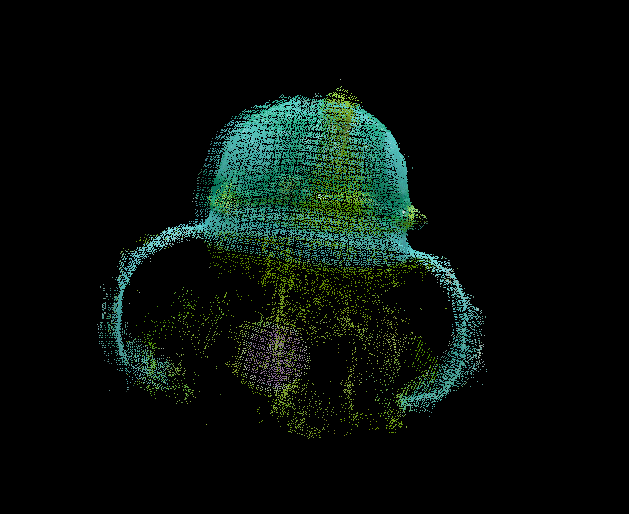
\includegraphics[width=10cm]{apc_model1}
  \caption{APC数据集中的3D模型}
  \label{fig:apc_model}
\end{figure}
模型点云的缺失,因此将点云投影到图像平面生成的mask也有部分缺失,尽管已经对生成的mask进行了一些滤波处理,但部分Mask还是有明显的缺失。

总体来说,尽管生成的ground truth的质量没有人工标注的ground truth质量好,但对本实验来说已经够用,并且相比人工标注这种半自动化的标注方式节省了大量时间和金钱成本。

workpiece数据集有三类物体,共2k组图片。该数据集与APC数据集最大的不同是,同一张图片中存在大量不同位姿的同种物体,并且三类物体都缺少纹理(textureless),因此Faster R-CNN和Mask R-CNN在该数据集上的表现理论上应该大大不如所设计的检测模块。部分数据集中的图片如图\ref{fig:wp_dataset}所示。
\begin{figure}[ht]
  \centering
  \subfloat{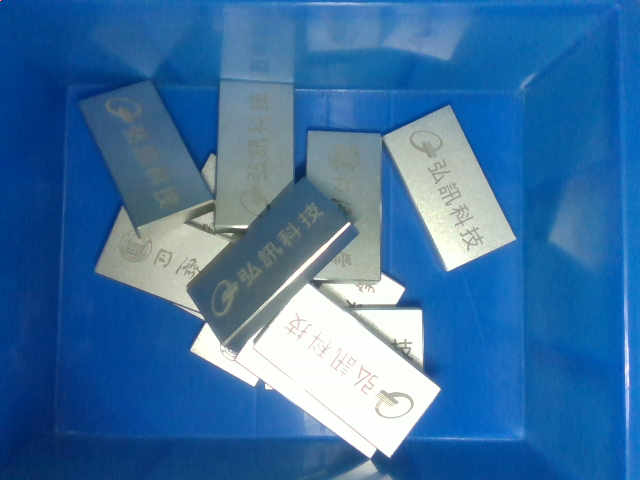
\includegraphics[width=3.5cm]{wp_color1}}
  \hskip0.2cm
  \subfloat{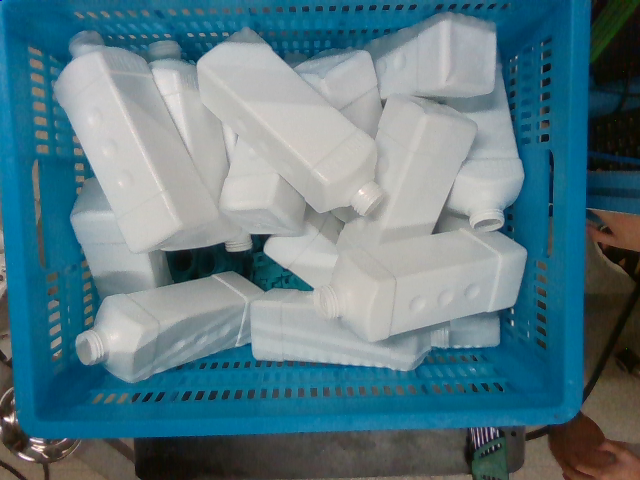
\includegraphics[width=3.5cm]{wp_color2}}
  \hskip0.2cm
  \subfloat{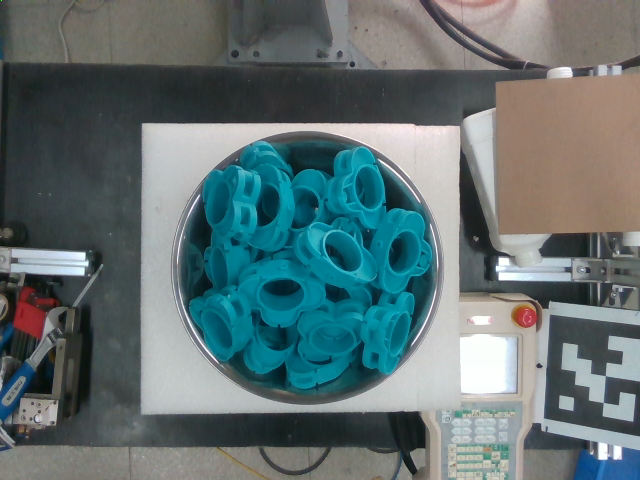
\includegraphics[width=3.5cm]{wp_color3}}
  \vfill
  \subfloat{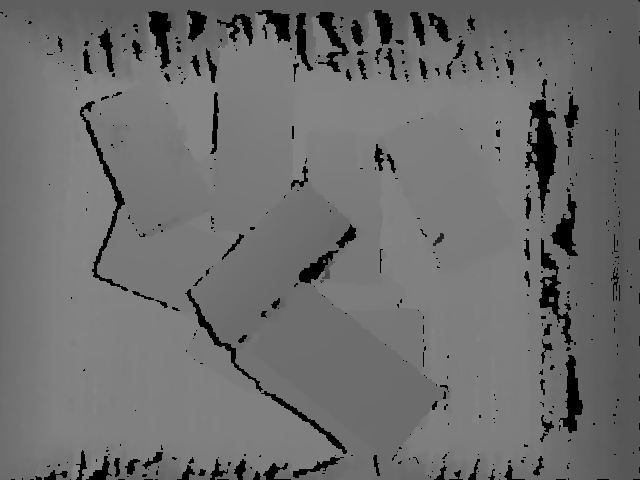
\includegraphics[width=3.5cm]{wp_depth1}}
  \hskip0.2cm
  \subfloat{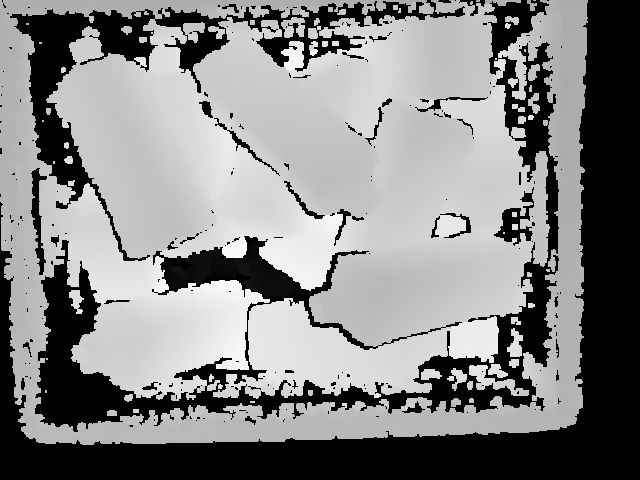
\includegraphics[width=3.5cm]{wp_depth2}}
  \hskip0.2cm
  \subfloat{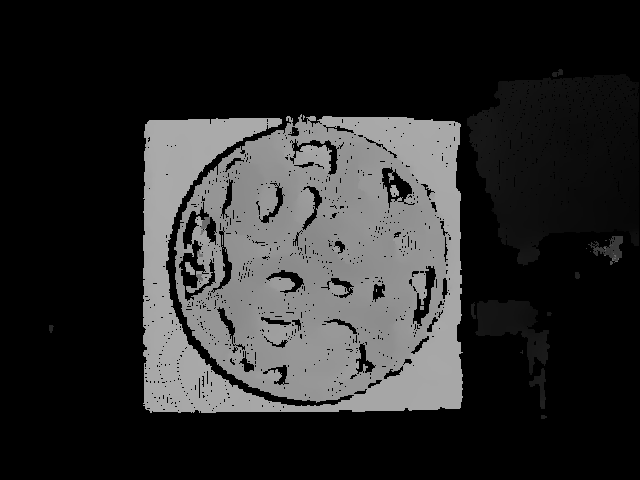
\includegraphics[width=3.5cm]{wp_depth3}}
  \caption{workpiece数据集部分图片}
  \label{fig:wp_dataset}
\end{figure}
workpiece数据集的ground truth由人工标定,其中据测试集中有的ground truth不仅包括了物体的Class,Mask,Bounding box,还有物体的位姿,并且由于三类物体都是工厂中的工件,因此也提供三类物体精确的CAD模型。

{\kai 算法实现}主要通过Tensorflow框架使用python语言实现,详细代码见Github项目地址\footnote{\url{https://github.com/freealong/Mask\_RCNN}}。

{\kai 评价的指标}主要是检测的精确度AP(Average Precision)以及算法的时间性能FPS。FPS是每秒能检测的图片数比较好理解,AP是BBox或者Mask交并比的精确度。具体地,如图\ref{fig:iou}所示,
\begin{figure}[ht]
  \centering
  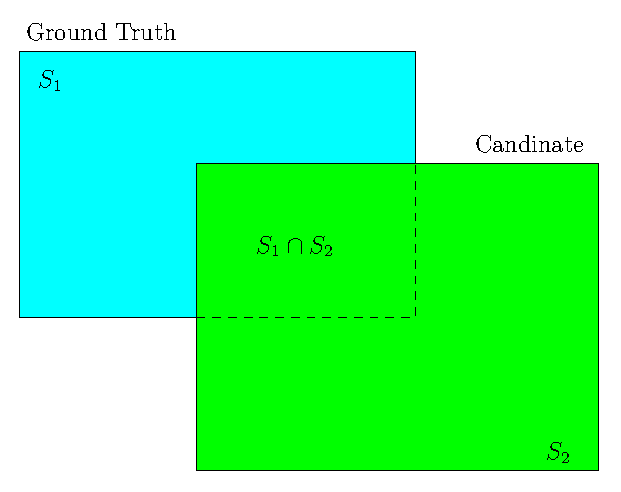
\includegraphics[width=8cm]{iou}
  \caption{Bounding Box交并比}
  \label{fig:iou}
\end{figure}
两个BBox的交并比定义为:
\begin{equation}
  IoU = \frac{S_1\cap S_2}{S_1\cup S_2}
\end{equation}
$AP_{0.5}$表示检测的结果与ground truth的交并比大于0.5的个数占总体检测个数的比例,显然定义精度的$IoU$大小会影响最终评价的质量,过小和过大的最小$IoU$都不能很好地反应算法的精缺度,因此将评价的主要精确度定义如下:
\begin{equation}
  AP = \frac{1}{10}\sum_{i=0}^{9}{AP_{0.5 + 0.5i}}
\end{equation}
检测结果换为Mask精确度的定义也类似,只需用Mask的交并比代替BBox的交并比。

{\kai 模型训练}在实验室的服务器上进行,服务器有两块Intel(R) Xeon(R) E5-2683 v3(2.00GHz)的CPU,4块TITAN X GPU。模型训练时为了减少训练时间,4块GPU都使用了。在APC数据集上,训练用了约6k组图片,剩下的1k多组图片用于测试,基于Faster R-CNN的检测模块训练用了40个小时左右,基于Mask R-CNN的检测模块用了48个小时左右;在workpiece数据集上,训练用了约1.6k组图片,剩下的400组图片用于测试,基于Faster R-CNN的检测模块训练用了30个小时左右,基于Mask R-CNN的检测模块用了36小时左右。

{\kai 实验结果}:
在APC数据集上,本文的检测模块与原始的Faster R-CNN和Mask R-CNN的精确度如表\ref{tab:ap1}所示,在测试集上的部分图片检测结果见图\ref{fig:apc_res}。
\begin{table}[ht]
  \centering
  \caption{APC数据集上的精确度}
    \begin{tabular}{cccccc}
      \toprule
      &input&output&$AP$&$AP_{0.5}$&$AP_{0.75}$ \\
      \midrule
      Faster R-CNN&RGB&bbox&33.26&56.29&34.03 \\
      \bf{Our method(based on Faster R-CNN)}&RGB+HHA&bbox&\bf{34.55}&\bf{57.99}&\bf{34.69} \\
      Mask R-CNN&RGB&mask&32.34&55.78&33.12 \\
      \bf{Our method(based on Mask R-CNN)}&RGB+HHA&mask&\bf{33.94}&\bf{56.45}&\bf{33.99} \\
      \bottomrule
    \end{tabular}
  \label{tab:ap1}
\end{table}
\begin{figure}[ht]
  \centering
  \subfloat{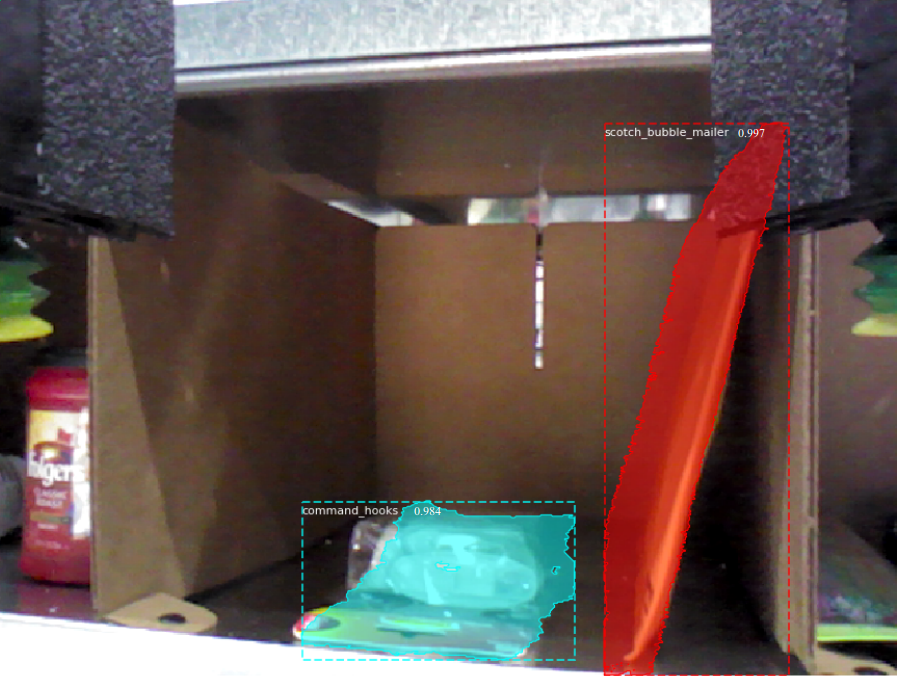
\includegraphics[width=4.5cm]{detect_apc_res1}}
  \hskip2pt
  \subfloat{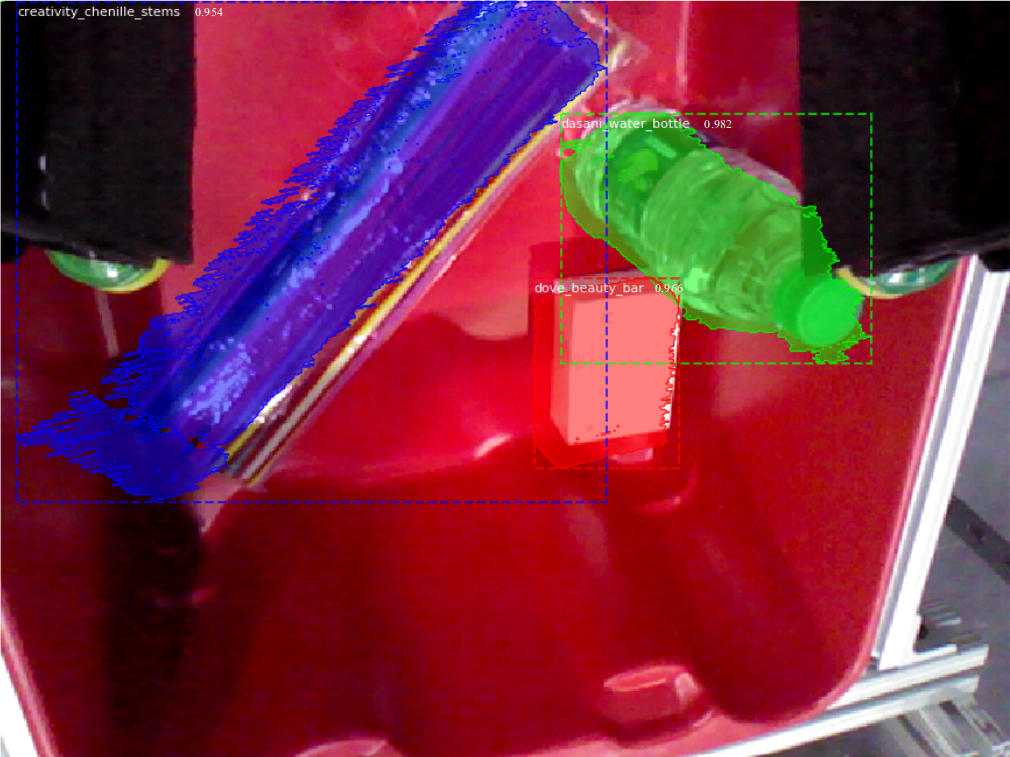
\includegraphics[width=4.5cm]{detect_apc_res2}}
  \hskip2pt
  \subfloat{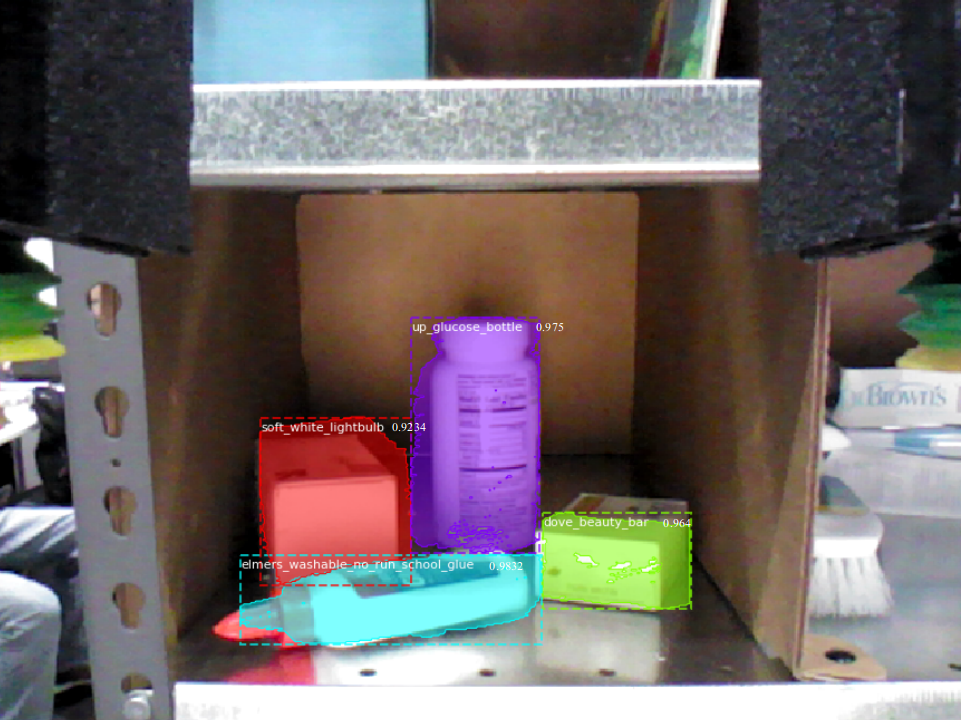
\includegraphics[width=4.5cm]{detect_apc_res3}}
  \caption{APC数据集上部分检测结果}
  \label{fig:apc_res}
\end{figure}
从表\ref{tab:ap1}中可以看出在APC数据集上本文基于Faster R-CNN所提出的方法相比Faster R-CNN的精确度提高了1.3个百分点左右,基于Mask R-CNN所提出的方法相比Mask R-CNN提高了0.8个百分点左右。整体来说对精确度的提高并不是十分明显,究其原因,从图\ref{fig:apc_dataset}可以看到APC数据集中的物体大多也是纹理丰富的,单从RGB图就可以训练出一个很好的模型,因此增加HHA通道,对模型精确度的提升十分有限,反而降低了算法的FPS。

在workpiece数据集上的检测精确度如表\ref{tab:ap2}所示,在测试集上的部分图片检测结果见图\ref{fig:wp_res}。
\begin{table}[ht]
  \centering
  \caption{workpiece数据集上的精确度}
    \begin{tabular}{cccccc}
      \toprule
      &input&output&$AP$&$AP_{0.5}$&$AP_{0.75}$ \\
      \midrule
      Faster R-CNN&RGB&bbox&18.78&37.49&19.46 \\
      \bf{Our method(based on Faster R-CNN)}&RGB+HHA&bbox&\bf{32.39}&\bf{56.37}&\bf{33.54} \\
      Mask R-CNN&RGB&mask&16.12&35.95&18.74 \\
      \bf{Our method(based on Mask R-CNN)}&RGB+HHA&mask&\bf{30.98}&\bf{53.74}&\bf{32.19} \\
      \bottomrule
    \end{tabular}
  \label{tab:ap2}
\end{table}
\begin{figure}[ht]
  \centering
  \subfloat{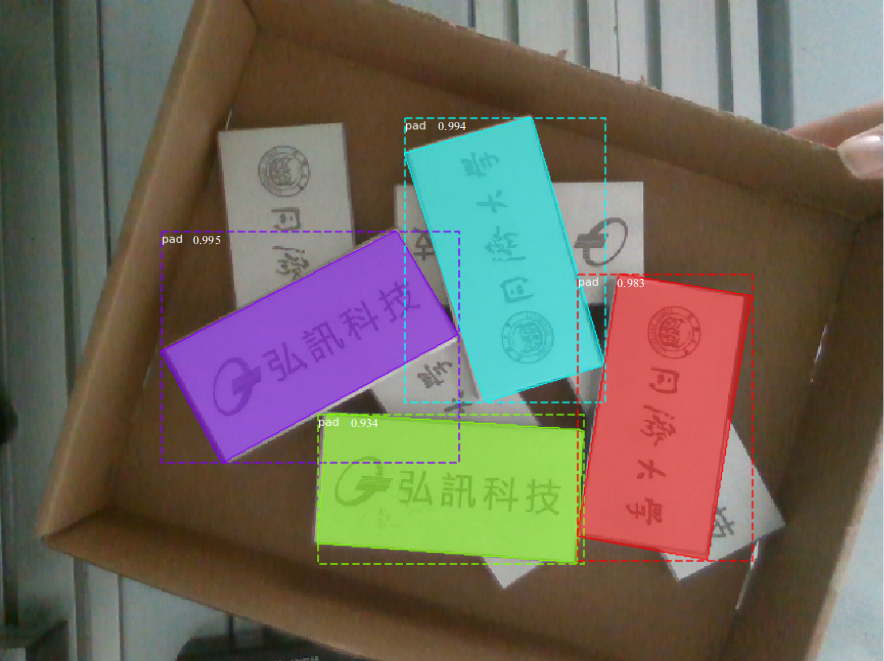
\includegraphics[width=4.5cm]{detect_wp_res1}}
  \hskip0.2cm
  \subfloat{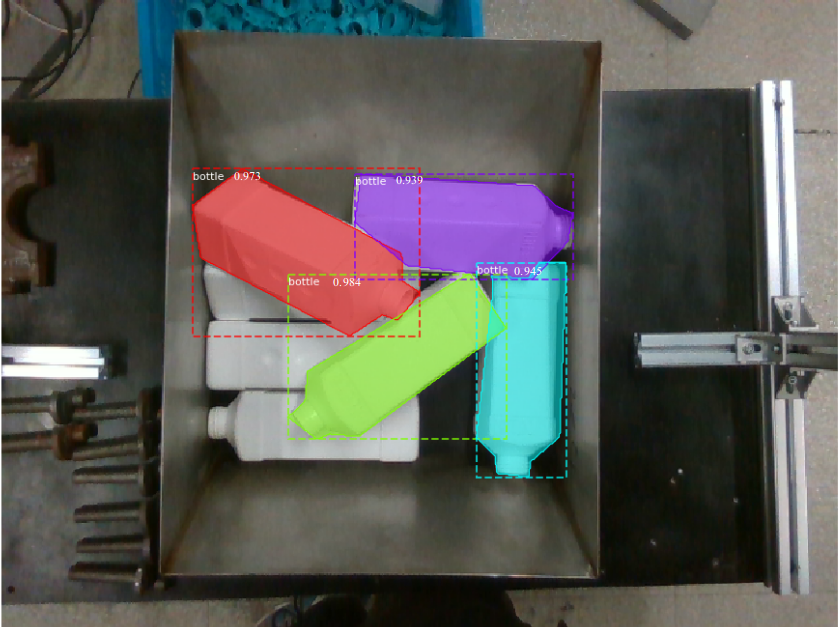
\includegraphics[width=4.5cm]{detect_wp_res2}}
  \hskip0.2cm
  \subfloat{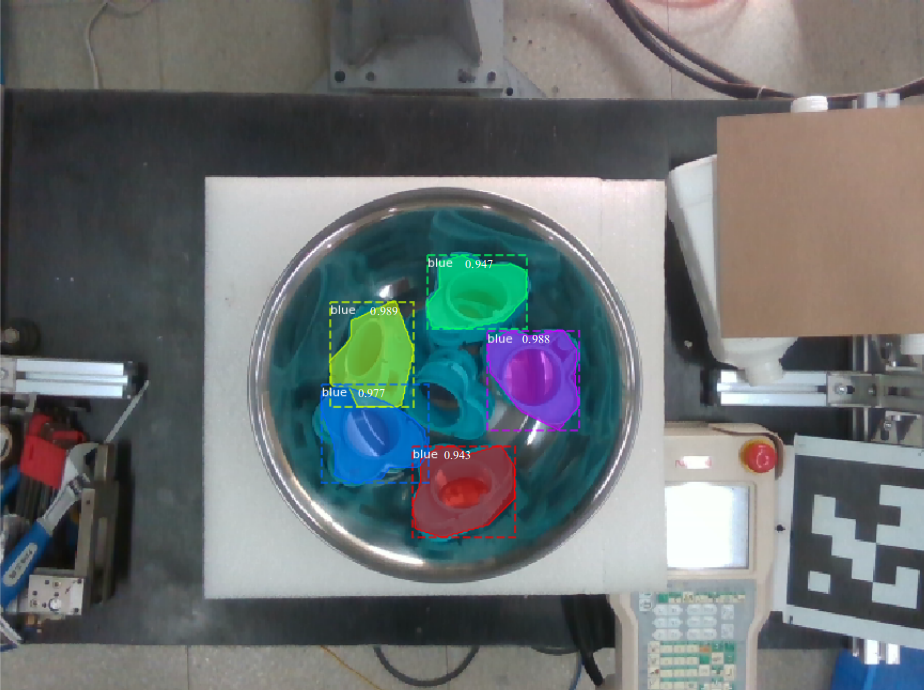
\includegraphics[width=4.5cm]{detect_wp_res3}}
  \caption{workpiece数据集上部分检测结果}
  \label{fig:wp_res}
\end{figure}
从表\ref{tab:ap2}可以看出在workpiece数据集上,本文基于Faster R-CNN所提出的检测模块相比Faster R-CNN的精确度提高了13.6个百分点左右,基于Mask R-CNN所提出的检测模块相比Mask R-CNN提高了约14.8个百分点。显然,本文所提出的检测模块在workpiece数据集上精确度相比原算法有了大大的提高,从图\ref{fig:wp_dataset}可以发现workpiece数据集中的图片包含的都是一些缺少纹理的物体,并且有大量同种物体混杂在一起,有时候人眼也很难从中区分单个目标,因此可能单从RGB图难以训练出一个准确率较高的模型来检测目标。而这些缺少纹理的大量物体在深度图,尤其是变换后的HHA图上十分容易区分出来,因此引入HHA后,增加了更多信息,最终训练得到的模型的准确度相比原算法有了巨大的提升。

所提出的检测模块的时间性能见表\ref{tab:fps},
由于两个数据集内图片的大小都是一样的,因此算法的时间性能在两个数据集上并不会有什么差异,因此表\ref{tab:fps}中直接统计了算法在两个数据集测试样本上FPS的平均值。从表\ref{tab:fps}可以看出本文所提出的检测模块与Faster R-CNN和Mask R-CNN相比,普遍具有更低的FPS,主要因为增加了HHA数据并且增加了STN模块。但考虑到本文算法的具体应用,适当降低的FPS并不会对具体使用造成什么影响。
\begin{table}[ht]
  \centering
  \caption{算法时间性能}
  \begin{tabular}{cc}
    \toprule
    &FPS \\
    \midrule
    Faster R-CNN&5.5 \\
    \bf{Our method(based on Faster R-CNN)}&\bf{3.2} \\
    Mask R-CNN&4.1 \\
    \bf{Our method(based on Mask R-CNN)}&\bf{2.5} \\
    \bottomrule
  \end{tabular}
  \label{tab:fps}
\end{table}

\section{匹配模块}
\label{sec:matcher}

\subsection{模块框架设计}
本文设计的匹配模块的框图如图\ref{fig:4pcs-pe}所示,
\begin{figure}[ht]
  \centering
  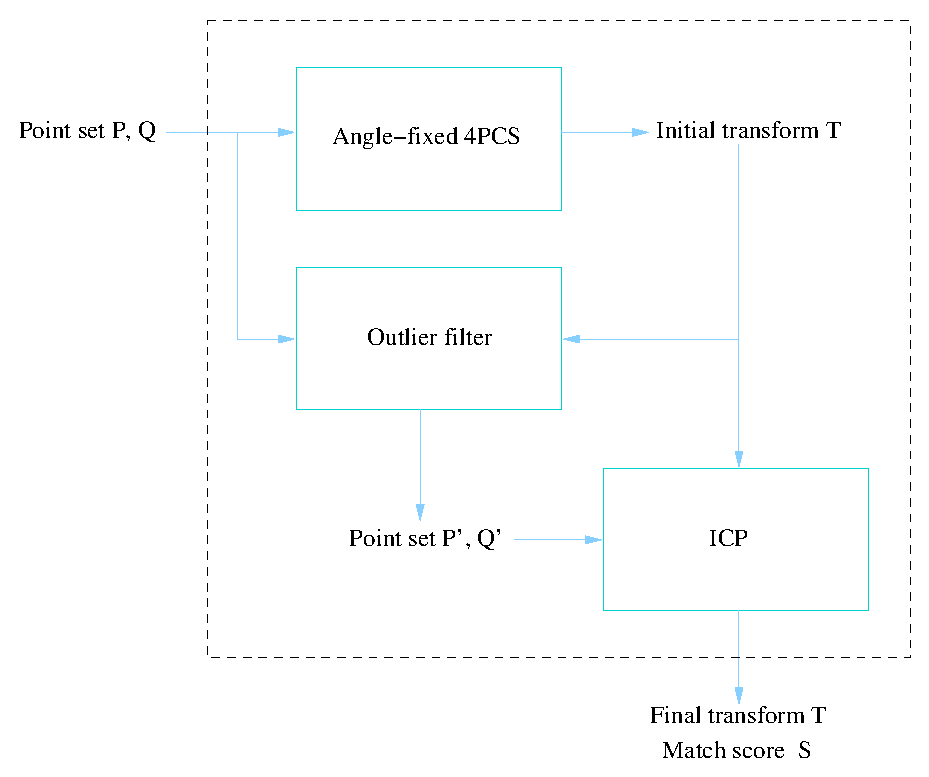
\includegraphics[width=12cm]{4pcs-pe}
  \caption{匹配模块框架}
  \label{fig:4pcs-pe}
\end{figure}
匹配模块的输入是两个点云(点集)\footnote{本文对点集(point set)与点云(point cloud)不做区分,都指包含坐标点的集合}$P$和$Q$,输出的是这两个点云之间的刚体变换$T$。

点云之间的匹配问题并不是一个新的问题,解决该问题的算法也有很多,尤其是近些年来,随着几何扫描相关技术的发展,如何将多次扫描或者多个设备采集的三维信息统一到一个坐标系下成为研究的热点,这些问题也是计算机几何学和计算机视觉中的基础问题。

其中一个比较流行的算法是通过使用稳定的局部几何描述子来匹配得到粗略的刚体变换,然后紧接着使用ICP算法\cite{besl1992method}迭代获取较为精确的刚体变换\cite{li2005multiscale}。这种算法的效果十分取决于所选取的描述子,通常一般的描述子对传感器噪声都比较敏感,尤其是一些低精度的传感器,常用的局部几何特征描述子有SHOT\cite{salti2014shot}、FFPH\cite{rusu2009fast}等;还有一种比较流行的方法是通过几何希哈方法从事先设置好的候选集中来选择合适的刚体变换\cite{wolfson1997geometric};一些随机算法,如RANSAC(Random Sample Consesue)\cite{bolles1981ransac}通常需要足够长的时间才能保证得到合适的解。

上述介绍的一些算法,有些对噪声的鲁棒性不强,有些时间复杂度极高,有些也难以处理部分重叠的情况,即点集$P$和$Q$之间只有一部分点集是相匹配的,因此难以实际直接应用到本文所需要解决的问题,其效果也难以让人满意。对此,本文基于4PCS(4-Points Congruent Sets)\cite{aiger20084}算法设计了有效解决点云匹配的匹配模块。

所设计的匹配模块首先针对4PCS算法的不足,对其进行改进,然后通过对离群点进行过滤和利用ICP算法进行迭代提升最终匹配的精度。从图\ref{fig:4pcs-pe}中可以看出所设计的匹配模块主要由三个部分组成:改进的4PCS算法(Angle-fixed 4PCS)、Outlier filter和ICP算法。改进的4PCS算法根据输入的两个点云输出两个点集之间的粗略的变换关系;Outlier filter根据改进的4PCS算法的输出对点集$P'$和$Q'$进行滤波,去掉一些离群点,用以提高下一步ICP算法的精度;ICP模块通过以改进后的4PCS算法输出的变换关系为初始值对滤波后的两个点集进行迭代求解最佳的刚体变换关系,输出最终的变换关系$T$和匹配的分数$S$,$T$也是目标的位姿,$S$是点云匹配误差的倒数,\ref{sec:matcher_exp}小节会具体介绍匹配误差。

\subsection{4PCS算法的改进}
介绍改进的4PCS算法之前,首先必须详细介绍一下4PCS算法。4PCS算法是用于求解LCP(Largest Common Pointset)问题的一个算法,LCP问题的定义如下:

{\kai LCP问题:给定两个点集$P$和$Q$,在给定距离误差$\delta$下,求解点集$P$的最大子集$P'$,使得$T(P')$和点集$Q$之间的距离在合适的距离度量下小于$\delta$,其中$T$是一个刚体变换。}

\begin{algorithm}
  \caption{4PCS算法}
  \label{alg:4pcs}
  \KwIn{Point sets $P$ and $Q$, measure level $\delta$}
  \KwOut{Rigid transform $T$}
  $h\leftarrow 0$\;
  \For {$i = 1$ to $L$} {
    $B\leftarrow$ SELECTCOPLANARBASE($P$)\;
    $U\leftarrow$ FINDCONGRUENT($B,Q,\delta$)\;
    \ForAll {4-points coplannar sets $U_i\in U$} {
      $T_i\leftarrow$ best rigid transform that aligns $B$ to $U_i$ in the least square sense\;
      Find $S_i\subseteq P$, such that $d(T_i(S_i), Q)\leq\delta$\;
    }
    $k\leftarrow arg\;\underset{i}{max}\left\{|S_i|\right\}$\;
    \If {$|S_k| > h$} {
      $h\leftarrow |S_k|$\;
      $T\leftarrow T_k$\;
    }
    \Return $T$\;
  }
  \BlankLine
  \BlankLine
  \BlankLine
  \BlankLine
  \SetKwProg{Def}{def}{:}{}
  \Def{FINDCONGRUENT($B:=\left\{\mathbf{b}_1,\mathbf{b}_2,\mathbf{b}_3,\mathbf{b}_4\right\},Q,\delta)$} {
    $d_1\leftarrow\;\parallel\mathbf{b}_1-\mathbf{b}_2\parallel$\;
    $d_2\leftarrow\;\parallel\mathbf{b}_3-\mathbf{b}_4\parallel$\;
    计算$R_1\equiv\left\{(\mathbf{p}_i,\mathbf{p}_j)\;|\;\mathbf{p}_i,\mathbf{p}_j\;\in Q\right\}$,使得$\parallel\mathbf{p}_i-\mathbf{p}_j\parallel\;\in [d_1-\delta,d_1+\delta]$\;
    计算$R_2\equiv\left\{(\mathbf{p}_i,\mathbf{p}_j)\;|\;\mathbf{p}_i,\mathbf{p}_j\;\in Q\right\}$,使得$\parallel\mathbf{p}_i-\mathbf{p}_j\parallel\;\in [d_2-\delta,d_2+\delta]$\;
    \ForAll {$r_{1i}\in R_1$} {
      计算与定量$r_1$和$r_2$相关的四个点$\left\{\mathbf{e}_{1i}^1,\mathbf{e}_{1i}^2,\mathbf{e}_{1i}^3,\mathbf{e}_{1i}^4\right\}$,记$\Pi(\mathbf{e}_{1i}^j)=r_{1i}$\;
    }
    对点集$\left\{\mathbf{e}_{1i}^j\right\}$在$\mathbb{R}^3$空间建立range tree的数据结构\;
    \ForAll {$r_{2i}\in R_1$} {
      计算与定量$r_1$和$r_2$相关的四个点$\left\{\mathbf{e}_{2i}^1,\mathbf{e}_{2i}^2,\mathbf{e}_{2i}^3,\mathbf{e}_{2i}^4\right\}$,记$\Pi(\mathbf{e}_{1i}^j)=r_{1i}$\;
    }
    $U'\leftarrow\varnothing$\;
    \ForAll {$\mathbf{e}_{2i}^j$} {
      在range tree中以$\delta$为领域检索点$\mathbf{e}_{2i}^j$附近的点,对于每个检索到的点$\mathbf{q}$,建立与$B$相对应的4个点的点集$U'\leftarrow\left\{U',(\Pi(\mathbf{q}),\Pi(\mathbf{e}_{2i}^j))\right\}$\;
    }
    \Return $U'$\;
  }
\end{algorithm}

4PCS算法具体的流程如\ref{alg:4pcs}所示,该算法输入两个点集$P$和$Q$,还有距离参数$\delta$,返回两个点集之间的刚体变换$T$。4PCS基于以下事实:{\kai 共面点集中定义的比例在仿射变换,包括刚体运动中保持不变。}举例来说,定义点集$X:=\left\{\mathbf{a},\mathbf{b},\mathbf{c},\mathbf{d}\right\}$,其中4个点不都在同一条直线上,设直线$ab$和$cd$相交于点$\mathbf{e}$,定义两个比例:
\begin{equation}
  \begin{array}{ccc}
    r_1& =& {\parallel \mathbf{a}-\mathbf{e}\parallel}/{\parallel \mathbf{a}-\mathbf{b}\parallel}\\
    r_2& =& {\parallel \mathbf{c}-\mathbf{e}\parallel}/{\parallel \mathbf{c}-\mathbf{d}\parallel}
  \end{array}
\end{equation}
则在仿射变换下所定义的$r_1$和$r_2$均保持不变,如图\ref{fig:4points}。
\begin{figure}[ht]
  \centering
  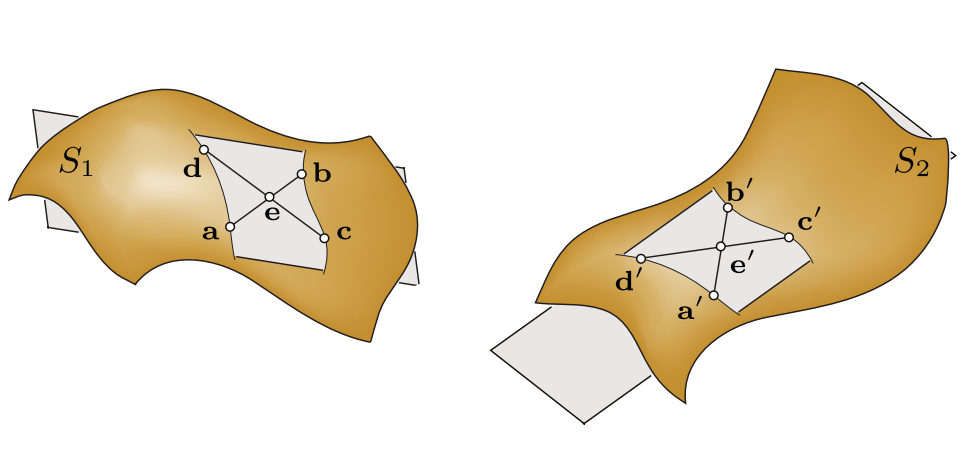
\includegraphics[width=12cm]{4points}
  \caption{4-points比例的仿射不变性}
  \label{fig:4points}
\end{figure}
如果曲面$S_1$和$S_2$匹配,并且4-points共面基在重叠区域,则$\mathbf{a},\mathbf{b},\mathbf{c},\mathbf{d}$对应的四个点$\mathbf{a}',\mathbf{b}',\mathbf{c}',\mathbf{d}'$也共面,并且
\begin{equation}
  \begin{array}{ccc}
    {\parallel \mathbf{a}'-\mathbf{e}'\parallel}/{\parallel \mathbf{a}'-\mathbf{b}'\parallel}&=&r_1\\
    {\parallel \mathbf{c}'-\mathbf{e}'\parallel}/{\parallel \mathbf{c}'-\mathbf{d}'\parallel}&=&r_2\\
  \end{array}
\end{equation}


4PCS算法另一个关键技术是使用了{\kai 宽基}(\emph{wide-base}),相比于一般的基,宽基中基的长度更长,如图\ref{fig:wide-base}所示,图片上半部分是使用宽基匹配的曲线,图片下半部分是使用一般的基匹配的曲线,显然,通过比较可以发现宽基相比普通基有更稳定的匹配结果,相关理论证明见文献\cite{goodrich1994practical}。
\begin{figure}[ht]
  \centering
  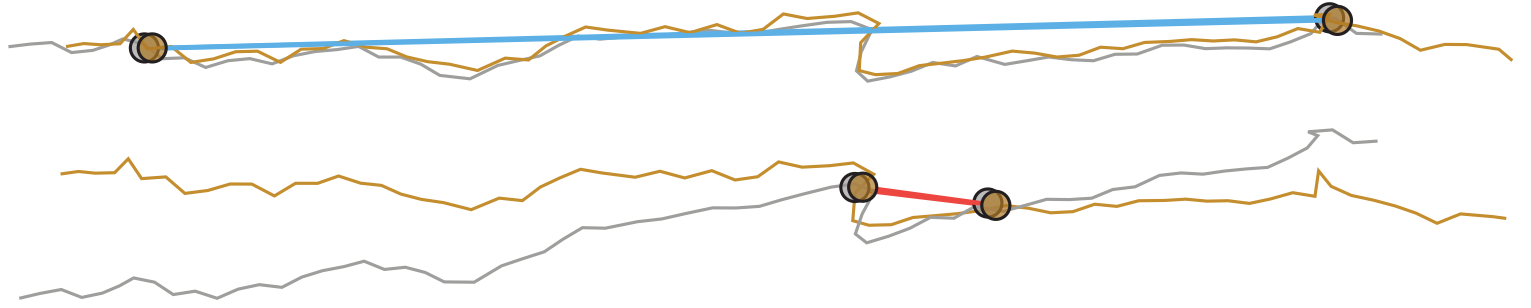
\includegraphics[width=14cm]{wide-base}
  \caption{宽基的匹配稳定性}
  \label{fig:wide-base}
\end{figure}

回到4PCS算法具体实现,算法的主体其实是一个RANSAC循环,每次循环首先会从点集$P$中挑选共面的宽基$B$,具体实现时,先从点集$P$中随机选取3个点,然后在剩下的点中选取第四个点构成共面的四点,第四个点的选取尽可能使得每个点之间的距离最大(因为我们要使用宽基),并且与前3个点近似共面(显然由于噪声的存在,完全共面并不现实),但如果第四个点选取的过远也会出现问题,因为如果宽基超过两个点集的重叠区域则难以匹配,因此当选以最大距离取宽基造成误差变大时以$f=1,0.5,0.25,\ldots$的比率降低最大距离来选取宽基。

在点集$P$中选取好宽基$B$后,算法下一步会在点集$Q$中通过4-points的仿射不变性找出所有与宽基$B$“全等”的基,构成集合$U$。在$Q$中选取基的方法见算法\ref{alg:4pcs}中的FINDCONGRUENT函数,函数首先使用基$B$中的点先定义两个仿射无关的比例,如图\ref{fig:findbase}中左边的图所示。
\begin{figure}[ht]
  \centering
  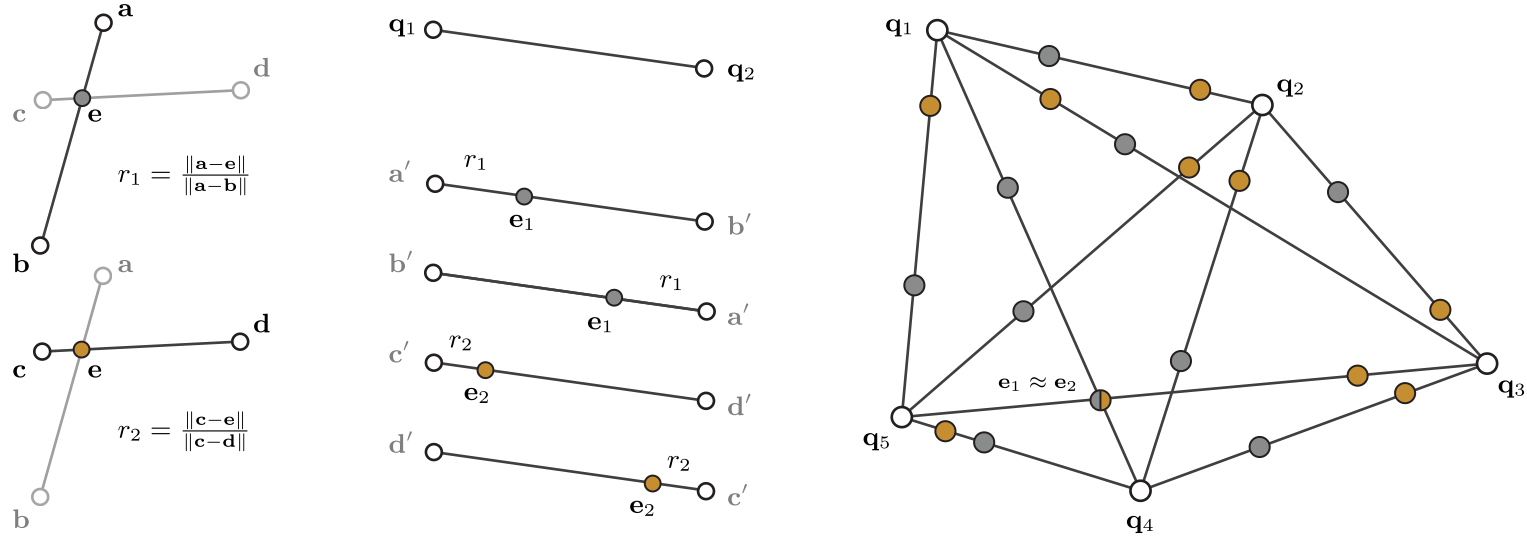
\includegraphics[width=15cm]{findbase}
  \caption{寻找近似“全等”的基示意图}
  \label{fig:findbase}
\end{figure}
假设在点集$Q$中找到两点$\mathbf{q}_1$和$\mathbf{q}_2$,并且$\left|\parallel \mathbf{q}_1-\mathbf{q}_2\parallel - \parallel \mathbf{a}-\mathbf{b}\parallel\right| \leq \delta$,则点$\mathbf{q}_1,\mathbf{q}_2$有可能与点$\mathbf{a}, \mathbf{b}$对应,则直线$\mathbf{a}\mathbf{b}$与$\mathbf{c}\mathbf{d}$相交的点$\mathbf{e}$的对应点可能为
\begin{equation}
  \mathbf{e}_1 = \mathbf{q}_1 + r1(\mathbf{q}_2-\mathbf{q}_1)
\end{equation}
或者
\begin{equation}
  \mathbf{e}_1 = \mathbf{q}_2 + r1(\mathbf{q}_1-\mathbf{q}_2)
\end{equation}
同理也可以根据$\mathbf{c},\mathbf{d}$的对应点(设为$\mathbf{q}_3, \mathbf{q}_4$)求得$\mathbf{e}$的对应点
\begin{equation}
  \mathbf{e}_2 = \mathbf{q}_3 + r1(\mathbf{q}_4-\mathbf{q}_3)
\end{equation}
或者
\begin{equation}
  \mathbf{e}_2 = \mathbf{q}_4 + r1(\mathbf{q}_3-\mathbf{q}_4)
\end{equation}
则当$\mathbf{e}_1\approx \mathbf{e}_2$时,$\mathbf{q}_1,\mathbf{q}_2,\mathbf{q}_3,\mathbf{q}_4$就是我们所要找的一组与点$\mathbf{a},\mathbf{b},\mathbf{c},\mathbf{d}$近似“全等”的基,如图\ref{fig:findbase}中右边图中的$\mathbf{q}_5,\mathbf{q}_3,\mathbf{q}_4,\mathbf{q}_1$。

具体实现时,当我们在点集$Q$中找出了所有可能的$\mathbf{e}_1$和$\mathbf{e}_2$后,找出其中近似相等的$\mathbf{e}_1$和$\mathbf{e}_2$可以通过range树\cite{arya1998optimal}来实现,对于大小为$n$的点集,range树的建立时间复杂度为$O(n\lg n)$,查询附近点的时间复杂度为$O(\lg n + k)$,其中$k$是查询到点的个数。

在$Q$中找出所有与基$B$近似“全等”的基后,下一步就是计算出最优的刚体变换$T$。对于$U$中的每个基$U_i$,我们可以利用最小二乘\cite{horn1987closed}的思想计算$B$到$U_i$的刚体变换$T_i$。得到刚体变换$T_i$后,我们将点集$P$进行变换$T_i$,然后对变换后的点集中的点在$Q$中查找最近点,统计最近点距离小于$\delta$的个数$S_i$,$S_i$也是评价$T_i$效果的分数,分数越高的$T_i$就是我们要求的最优刚体变换$T$。

仔细研究4PCS算法,可以发现从点集$Q$中提取的基与$B$并不是全等的,如图\ref{fig:4pcs-flaw}所示,
\begin{figure}[ht]
  \centering
  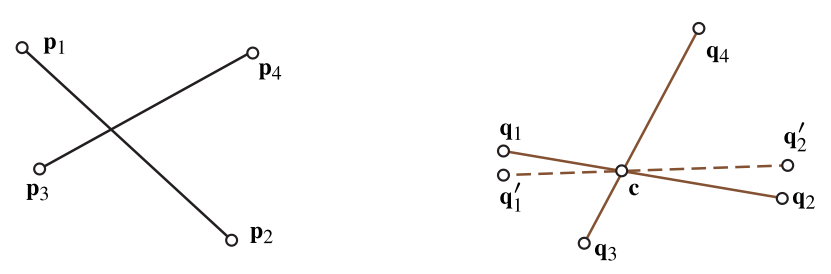
\includegraphics[width=12cm]{4pcs-flaw}
  \caption{4PCS中"全等“的基}
  \label{fig:4pcs-flaw}
\end{figure}
将线段$\mathbf{q}_1\mathbf{q}_2$绕交点转动一定角度后便不再与原基全等,但是4PCS仍然会找出点$\mathbf{q}_1',\mathbf{q}_2',\mathbf{q}_3,\mathbf{q}_4$作为与$\mathbf{p}_1',\mathbf{p}_2',\mathbf{p}_3,\mathbf{p}_4$全等的基。这一缺点会导致4PCS算法需要更多的求解时间,并且还有可能影响最终的匹配结果。因此,对4PCS改进去除这些与原基不是全等的基很有必要。改进后的算法如算法\ref{alg:a4pcs}所示,与原算法的区别在于,在FINDCONGRUENT函数后面增加了滤去不全等的基的步骤FILTERCONGRUENT函数。FINDCONGRUENT函数输入原基$B$、在$Q$中找到的与$B$全等的基的集合,以及允许的角度阈值$\epsilon$,然后通过比较基中两个向量之间的点积来判断角度是否近似相等,但由于我们无法确定向量的方向,即无法确定点$\mathbf{b}_1$是与$\mathbf{q}_1$对应还是与$\mathbf{q}_2$对应,因此$U$中基的两个向量之间的角度可能与$B$中相差180度。
\begin{algorithm}
  \caption{改进的4PCS算法}
  \label{alg:a4pcs}
  \KwIn{Point sets $P$ and $Q$, distance tolerance $\delta$, angle tolerance $\epsilon$}
  \KwOut{Rigid transform $T$}
  $h\leftarrow 0$\;
  \For {$i = 1$ to $L$} {
    $B\leftarrow$ SELECTCOPLANARBASE($P$)\;
    $U\leftarrow$ FINDCONGRUENT($B,Q,\delta$)\;
    $U\leftarrow$ FILTERCONGRUENT($B,U,\epsilon$)\;
    \ForAll {4-points coplannar sets $U_i\in U$} {
      $T_i\leftarrow$ best rigid transform that aligns $B$ to $U_i$ in the least square sense\;
      Find $S_i\subseteq P$, such that $d(T_i(S_i), Q)\leq\delta$\;
    }
    $k\leftarrow arg\;\underset{i}{max}\left\{|S_i|\right\}$\;
    \If {$|S_k| > h$} {
      $h\leftarrow |S_k|$\;
      $T\leftarrow T_k$\;
    }
    \Return $T$\;
  }
  \BlankLine
  \BlankLine
  \BlankLine
  \BlankLine
  \SetKwProg{Def}{def}{:}{}
  \Def{FILTERCONGRUENT($B:=\left\{\mathbf{b}_1,\mathbf{b}_2,\mathbf{b}_3,\mathbf{b}_4\right\},U,\epsilon)$} {
    $U'\leftarrow \varnothing$\;
    $a\leftarrow \overrightarrow{\mathbf{b}_1\mathbf{b}_2}\cdot \overrightarrow{\mathbf{b}_3\mathbf{b}_4}$\;
    \ForAll {$U_i:=\left\{\mathbf{q}_1,\mathbf{q}_2,\mathbf{q}_3,\mathbf{q}_4\right\}\in U$} {
      $a'\leftarrow \overrightarrow{\mathbf{q}_1\mathbf{q}_2}\cdot \overrightarrow{\mathbf{q}_3\mathbf{q}_4}$\;
      \If {$a'\in [a-\epsilon,a+\epsilon]\cup [-a-\epsilon,-a+\epsilon]$} {
        $U'\leftarrow \left\{U',U_i\right\}$\;
      }
    }
    \Return $U'$\;
  }
\end{algorithm}

\subsection{匹配精度优化}
实验表明,经过改进的4PCS算法输出的刚体变换$T$的精度不高,所以,所设计的匹配模块在改进的4PCS算法后面通过滤波和迭代来提升最终匹配的精度。

实际要匹配的两个点云往往不是完全重合的,也就是说两个点云匹配的时候有许多离群点,尤其是目标点云由BBox分割得到的情况,如图\ref{fig:outlier-pointcloud}所示,
\begin{figure}[ht]
  \centering
  \subfloat[目标3D模型转化的点云]{
    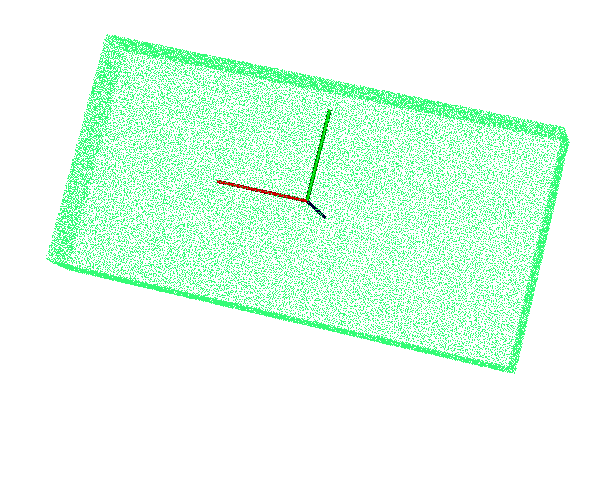
\includegraphics[width=6cm]{object-cloud}
  }
  \hskip1cm
  \subfloat[由BBox分割得到的点云]{
    \includegraphics[width=6cm]{target-cloud}
  }
  \caption{实际要匹配的两个点云}
  \label{fig:outlier-pointcloud}
\end{figure}
由BBox分割得到的点云由许多点并不与目标3D模型相匹配,将这些离群点滤去有助于提高最终的匹配精度,因此本文设计了Outlier filter模块用于滤去这些离群点,具体的算法如\ref{alg:outlier-filter}所示。
\begin{algorithm}[ht]
  \caption{Outlier filter算法}
  \label{alg:outlier-filter}
  \KwIn{Point sets $P$ and $Q$, Initial transform $T$, Distance tolerance $\delta$}
  \KwOut{Point sets $P'$ and $Q'$}
  $P'\leftarrow P$\;
  $Q'\leftarrow \varnothing$\;
  \ForAll {point $\mathbf{p}_i\in P$} {
    $\mathbf{p}_i\leftarrow T(\mathbf{p}_i)$\;
  }
  对点集$P$在$\mathbb{R}^3$空间建立kd树的数据结构\;
  \ForAll {point $\mathbf{q}_i\in Q$} {
    在kd树中检索出距离点$\mathbf{q}_i$最近的点$\mathbf{p}$\;
    $d\leftarrow\;\parallel\mathbf{q}_i-\mathbf{p}\parallel$\;
    \If {$d \leq \delta$} {
      $Q'\leftarrow \left\{Q', \mathbf{q}_i\right\}$\;
    }
  }
  \Return $P'$,$Q'$\;
\end{algorithm}
算法输入点集$P$和$Q$,需要参数初始刚体变换$T$,以及允许的距离误差$\delta$,由于点集$P$是由物体的CAD模型转换过来的,因此不对其进行滤波,只对点集$Q$进行离群点去除。具体方法是,首先使用$T$对点集$P$进行刚体变换;然后对变换后的点集建立kd树,建立kd树的目的是为了快速在点集$P$中找到距离某点最近的点,其查找的时间复杂度为$O(kN^{1-1/k})$,其中$k$是所建立kd树的维数,显然对于三维空间中点集为3,$N$是建立的kd树的节点个数;建立好kd树后,对点集$Q$中的每个点在kd树中找到与之距离最近的点,如果两点间的距离大于所设的参数$\delta$,则在点集Q中去除该点。实际运行Outlier filter算法的效果如图\ref{fig:outlier-filter}所示。
\begin{figure}[ht]
  \centering
  \includegraphics[width=15cm]{outlier-filter}
  \caption{离群点滤波效果图}
  \label{fig:outlier-filter}
\end{figure}

在滤去离群点后,为了提升匹配精度,我们使用ICP算法对滤去离群点后的点云进行迭代匹配。ICP算法本质上是基于最小二乘法的最优配准方法。该算法重复进行选择对应关系点对,计算最优刚体变换,直到满足正确配准的收敛精度要求。由于ICP算法是一种迭代算法,因此只要时间允许便可以获取足够精度的解,但也正因为如此,ICP也容易陷入局部最优解。本文充分考虑了ICP算法的这个特点,通过改进的4PCS算法给出初始的刚体变换来避免ICP算法陷入局部最优解,同时通过迭代来提高最后输出的刚体变换精度。

ICP算法的原理很简单,给定两个点集$P_n:=\left\{\mathbf{p}_1,\mathbf{p}_2,\ldots,\mathbf{p}_n\right\}$和$Q_m:=\left\{\mathbf{q}_1,\mathbf{q}_2,\ldots,\mathbf{q}_m\right\}$,以及初始旋转变换$R$和平移变换$t$,以及迭代结束额距离误差$\delta$,ICP算法迭代步骤如下:
\begin{itemize}
\item {\kai 步骤1:}根据当前$R$和$t$,对于点集$P_n$中的每个点在$Q_m$中找出距离最近的点,构成点集$Q_n$;
\item {\kai 步骤2:}计算$P_n$和$Q_n$之间的距离的均方根误差:
  \begin{equation}
    E(R,t) = \frac{1}{n}\sum_{i=1}^n{\parallel \mathbf{q}_i - R\mathbf{p}_i - t\parallel}
  \end{equation}
  通过奇异值分解求得使得$E(R,t)$最小的$R'$和$t'$;
\item {\kai 步骤3:}如果$E(R,t) < \delta$,结束迭代;否则$R\leftarrow R'$,$t\leftarrow t'$,跳转至步骤1。
\end{itemize}

ICP算法的迭代过程还是相对来说十分简单的,唯一需要思考一下的是如何求得最小化$E(R,t)$的$R'$和$t'$,通过奇异值分解求解$R'$和$t'$的方法如下:

首先,记
\begin{equation}
  \left\{
  \begin{array}{ccccc}
  P_n'& = &\left\{\mathbf{p}_i-\mathbf{\mu}_p \;|\; \forall \mathbf{p}_i \in P_n\right\}&:=&\left\{\mathbf{p}'_i\right\}\\
  Q_n'& = &\left\{\mathbf{q}_i-\mathbf{\mu}_q \;|\; \forall \mathbf{q}_i \in Q_n\right\}&:=&\left\{\mathbf{q}'_i\right\}
  \end{array}
  \right.
\end{equation}
其中
\begin{equation}
  \left\{
    \begin{array}{ccc}
      \mathbf{\mu}_p&=&\frac{1}{n}\sum_{i=1}^n{\mathbf{p}_i}\\
      \mathbf{\mu}_q&=&\frac{1}{n}\sum_{i=1}^n{\mathbf{q}_i}
    \end{array}
  \right.
\end{equation}
再另
\begin{equation}
  W = \sum_{i=1}^n{\mathbf{p}_i'(\mathbf{q}_i')^T}
\end{equation}
然后对矩阵$W$进行奇异值分解:
\begin{equation}
  W = U\Sigma V^T
\end{equation}
则
\begin{equation}
  \left\{
    \begin{array}{ccc}
      R'&=&UV^T \\
        t'&=&\mathbf{\mu}_p-R'\mathbf{\mu}_q
    \end{array}
    \right.
\end{equation}

\subsection{匹配模块实验}
\label{sec:matcher_exp}
为了评价所设计的匹配模块,考察其匹配精度以及时间性能,本文通过实验,与其他同类匹配算法相比较,验证了所设计的匹配模块在匹配精确度和时间上的优势。

{\kai 实验内容}:
实验在多个点云匹配的数据集上测试了所设计的匹配模块和一个基于局部特征描述子和RANSAC的算法LD-RANSAC\cite{li2005multiscale}。数据集中的点云数据有从激光扫描获取的、深度摄像头采集的、双目摄像头重构的,并且里面的模型也多种多样,有人造物、纹理缺少的物体,光滑的物体,粗糙的物体等。用来作对比的LD-RANSAC算法使用了基于spin-image的描述子\cite{johnson1999using},LD-RANSAC的具体实现直接使用了PCL(Point Cloud Library)中的相关代码,人工配置了算法的参数以达到较好的匹配效果。

实验主要考察点云匹配的误差以及算法的运行时间,点云匹配的误差定义为两个点云之间的RMS误差:
\begin{equation}
  E = \sqrt{\frac{1}{N}\sum_{i=1}^{N}{\min_{p_j\in T(P)}\norm{q_i-p_j}^2}}
\end{equation}
显然RMS误差越小,点云的匹配效果越好,精度越高。

{\kai 实验结果}:
为了考察算法的精度,通过对输入数据增加高斯噪声,来观察算法在不同大小噪声下的RMS误差,所设计的匹配模块和LD-RANSAC算法的RMS误差随高斯噪声方差的变化曲线如图\ref{fig:err-noise}所示。
\begin{figure}[ht]
  \centering
  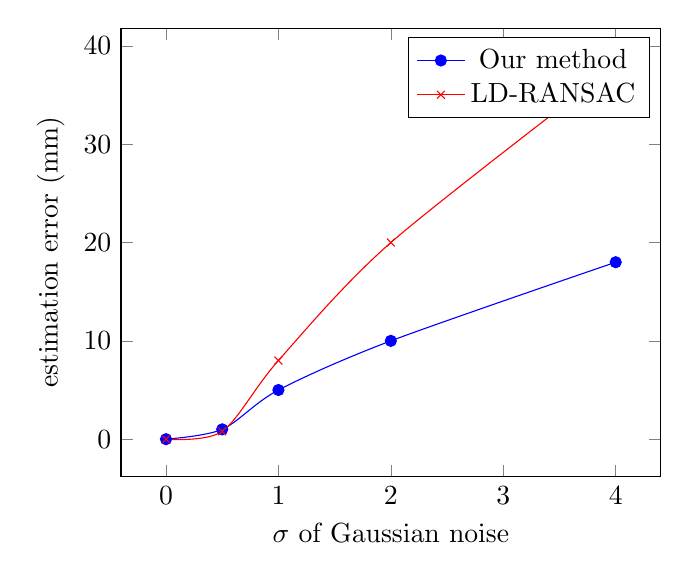
\begin{tikzpicture}
    \begin{axis}[xlabel=$\sigma$ of Gaussian noise, ylabel=estimation error (mm)]
      \addplot[smooth, mark=*, blue] plot coordinates {
        (0, 0)
        (0.5,1)
        (1, 5)
        (2, 10)
        (4, 18)
      };
      \addlegendentry{Our method}
      \addplot[smooth, mark=x, red] plot coordinates {
        (0, 0)
        (0.5,0.8)
        (1, 8)
        (2, 20)
        (4, 38)
      };
      \addlegendentry{LD-RANSAC}
    \end{axis}
  \end{tikzpicture}
  \caption{匹配误差随噪声变化曲线}
  \label{fig:err-noise}
\end{figure}
图中可以看出本文的方法比LD-RANSAC算法有更小的误差,并且对噪声也具有高强的鲁棒性。

为了考察算法的时间性能,通过对输入数据进行降采样(uniform sampling),变化uniform sampling的采集间距来变化输入点云的数量大小,不同点云数量大小下算法的运算时间的变化曲线如图\ref{fig:time-size}所示。
\begin{figure}[ht]
  \centering
  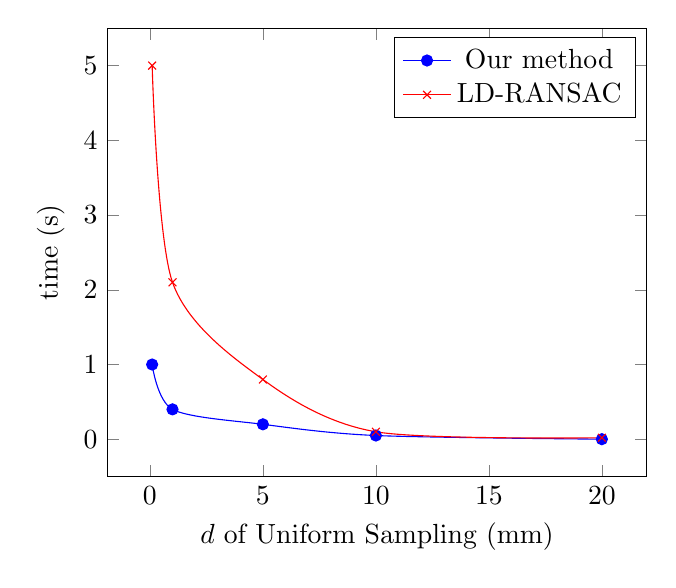
\begin{tikzpicture}
    \begin{axis}[xlabel=$d$ of Uniform Sampling (mm), ylabel=time (s)]
      \addplot[smooth, mark=*, blue] plot coordinates {
        (0.1, 1)
        (1,0.4)
        (5, 0.2)
        (10, 0.05)
        (20, 0.001)
      };
      \addlegendentry{Our method}
      \addplot[smooth, mark=x, red] plot coordinates {
        (0.1, 5)
        (1,2.1)
        (5, 0.8)
        (10, 0.1)
        (20, 0.02)
      };
      \addlegendentry{LD-RANSAC}
    \end{axis}
  \end{tikzpicture}
  \caption{匹配时间随点云数量大小变化曲线}
  \label{fig:time-size}
\end{figure}
图中可以看出本文所设计的方法的运算时间比LD-RANSAC少,并且随着点云数量的增加其运算时间的差距越来越大。

综上,本文所设计的匹配方法相比LD-RANSAC算法具有更高的匹配精度,对噪声的鲁棒性也更强,并且算法的时间复杂度也更小。

\section{3D-MRAI算法流程}
设计完检测模块和匹配模块后,整个3D-MRAI算法就比较简单了,其完整的算法流程如算法\ref{alg:3d-mrai}所示。
\begin{algorithm}
  \caption{3D-MRAI算法}
  \label{alg:3d-mrai}
  \KwIn{RGB Image $I$, Depth Map $D$, CAD Models $M$}
  \KwOut{Set of Pose and Class $Res$}
  $Res\leftarrow \varnothing$\;
  $P\leftarrow \varnothing$\;
  \ForAll {$M_i\in M$} {
    $P\leftarrow \left\{P, CAD2PointCloud(M_i)\right\}$\;
  }
  $H = Depth2HHA(D)$\;
  $Q = Depth2PointCloud(D)$\;
  $Mask, Class \leftarrow DetectModule(I, H)$\;
  \ForAll {$m_i\in Mask, c_i\in Class$} {
    $Q_i \leftarrow Crop(Q, m_i)$\;
    $P_i \leftarrow P(c_i)$\;
    $T_i,S_i\leftarrow MatchModule(P_i, Q_i)$\;
    \If {$S_i > S_{min}$} {
      $Res\leftarrow \left\{Res, \left[T_i, c_i\right]\right\}$\;
    }
  }
  \Return $Res$
\end{algorithm}

3D-MRAI算法首先会将目标的CAD模型转为匹配所需的点云。具体如何转换的话,基本思想是参考Uniform Sampling算法,Uniform Sampling算法的核心思想是以3D栅格中所有点的质心代替这些点,从而达到降采样。类似地,对于CAD模型也建立3D栅格,但由于无法获得3D栅格总所有点,因此判断CAD模型是否穿过3D栅格,如果穿过3D栅格,则在该3D栅格中心出增加一个点。显然3D栅格的边长越大,转换后的点云数量越小,精度越低,考虑到所使用相机生成点云的精度,因使CAD模型转换后的点云的精度与相机采集的点云的精度近似,实际取3D栅格边长为1mm,一个实际工件的CAD模型和以1mm为边长进行采样转换后的模型点云如图\ref{fig:model-pc}所示。
\begin{figure}[ht]
  \centering
  \subfloat[原CAD模型]{\includegraphics[width=7cm]{object-model}}
  \hskip1cm
  \subfloat[转换后点云]{\includegraphics[width=6cm]{object-pointcloud}}
  \caption{CAD模型和转换后的点云}
  \label{fig:model-pc}
\end{figure}

然后3D-MRAI算法会通过深度图计算HHA图和点云,由深度图计算HHA图的算法上文已经详细叙述过了,此处不再复述;将深度图变换为点云这一步则相对简单,只要通过深度摄像头的内参矩阵反投影到三维空间即可,详细见第~\ref{chap:rgbd}~章中RGB-D相机的数学模型。

处理完这些数据后,输入RGB图像和HHA图到检测模块,通过检测模块得到目标物体的BBox/Mask。然后根据BBox/Mask从深度图对应的点云中抠出目标点云,由于深度图转换的点云是有序的,因此BBox/Mask在深度图中的索引坐标与深度图转换的点云的索引坐标是一致的,只要将点云中对应的点提取出来就行,并滤去无效的点然后适当降采样即可,尽管滤波和降采样之后的目标点云是无序的,但后续匹配算法并不需要输入点云有序,而且降采样后点云数量减少,将会减少后续匹配算法的时间。


裁剪得到目标物体的点云$Q_i$后,找出对应物体的CAD模型转换的点云$P_i$,将$P_i$和$Q_i$输入到匹配模块,即可得到CAD模型到目标点云之间的刚体变换$T_i$,由于CAD模型坐标系与相机坐标系重叠,因此将矩阵$T$转换为$X,Y,Z,r,p,y$就是目标点云在相机坐标系下的位姿Pose,最后将所有匹配得到的结果与目标检测的结果组合,并滤去匹配或检测分数较低的结果。

\section{3D目标位姿估计实验}
为了评价所提出的3D-MRAI的性能,设计了3D目标位姿估计的实验,并与文献\cite{hinterstoisser2012model}所提出的基于LINEMOD算法的3D目标位姿估计框架相比较。
\subsection{数据集}
实验所使用的数据集是workpiece数据集,前文已经部分介绍过了,该数据集是在实验室采集的三类物体,检测模块实验中所用workpiece数据集中的ground truth是物体的种类、BBox和Mask,workpiece数据集中测试集中的图片的ground truth除了物体的种类、BBox和Mask,还有物体的位姿,物体的位姿是通过在物体旁固定标定板采集的。具体方法是,通过固定标定板在目标物体旁,我们可以记录标定板到目标的刚体变换关系$T_1$,然后我们通过彩色摄像头可以检测出标定板的位姿$T_2$,则物体的位姿可以通过下式得到
\begin{equation}
  T = T_2T_1
\end{equation}

\subsection{实验内容}
为了有效的评价3D-MRAI算法,我们先定义一个合适的评价指标{\kai 姿态误差}:
\begin{equation}
  m = {\underset{\mathbf{x}\in M}{avg}} \; {\parallel (R\mathbf{x}+t) - (\tilde{R}\mathbf{x}+\tilde{t})\parallel}
\end{equation}
其中$M$表示算法运行结果得到的物体种类对应的CAD模型转换得到的点云,$R$和$t$分别表示从ground truth物体位姿分解得到的旋转变换和平移变换,$\tilde{R}$和$\tilde{t}$分别表示从算法运行结果得到的物体位姿分解得到的旋转变换和平移变换。显然,如果算法运行结果和ground truth越接近,所定义的姿态误差就越小。对于一些对称的物体(如圆柱体的被子),显然不同角度下相机看到的目标物体可能近似,会造成算法运行的结果正确的情况下与ground truth相差很大,造成姿态误差很大,与我们所定义的评价指标的宗旨相违背。因此,针对一些对称的物体,重新定义姿态误差为
\begin{equation}
  m = {\avg_{\mathbf{x}_1\in M}} \; {\min_{\mathbf{x}_2\in M}} \; \norm{(R\mathbf{x}_1+t) - (\tilde{R}\mathbf{x}_2+t)}
\end{equation}
此外,如果$k_md>m$,我们就认为目标物体准确检测到了,并且估计的位姿正确,其中$d$是目标物体对应模型的直径,$k_m$是系数。因此,还可以定义一个正确检测目标并正确估计目标位姿的准确率。

实验在workpiece数据集的测试集上分别运行了3D-MRAI和文献\cite{hinterstoisser2012model}中的基于LINEMOD算法的检测框架,运行实验的计算机有两块Intel(R) Xeon(R) E5-2683 v3(2.00GHz)的CPU,4块TITAN X GPU,由于3D-MRAI有深度神经网络所以使用了一块GPU和一块CPU,Hinterstorisser等人的算法不需要GPU,只使用了一块CPU。

\subsection{实验结果}
\begin{figure}[ht]
  \centering
  \subfloat{\includegraphics[height=3.4cm]{3dmrai-res1}}
  \hskip0.2cm
  \subfloat{\includegraphics[height=3.4cm]{3dmrai-res2}}
  \hskip0.2cm
  \subfloat{\includegraphics[height=3.4cm]{3dmrai-res3}}
  \caption{3D-MRAI运算结果可视化图}
  \label{fig:3dmrai-res}
\end{figure}
3D-MRAI算法在workpiece数据集上一些测试用例的运算结果可视化如图\ref{fig:3dmrai-res}所示。变化系数$k_m$,根据3D-MRAI和Hinterstoisser等人的算法在测试集上的运行结果,统计算法的准确率如表\ref{tab:mrai}所示。
\begin{table}[ht]
  \centering
  \caption{3D-MRAI和Hinterstorisser等人的算法准确率}
  \begin{tabular}{ccccccc}
    \toprule
    $k_m[\%]$&5&7&9&11&13&15\\
    \midrule
    Hinterstorisser et al.&75.63& 83.84& 89.13& 93.48& 96.83&98.12\\
    \bf{3D-MRAI}&95.12& 97.35& 98.10& 98.69& 99.22& 100.00\\
    \bottomrule
  \end{tabular}
  \label{tab:mrai}
\end{table}
\begin{figure}[ht]
  \centering
     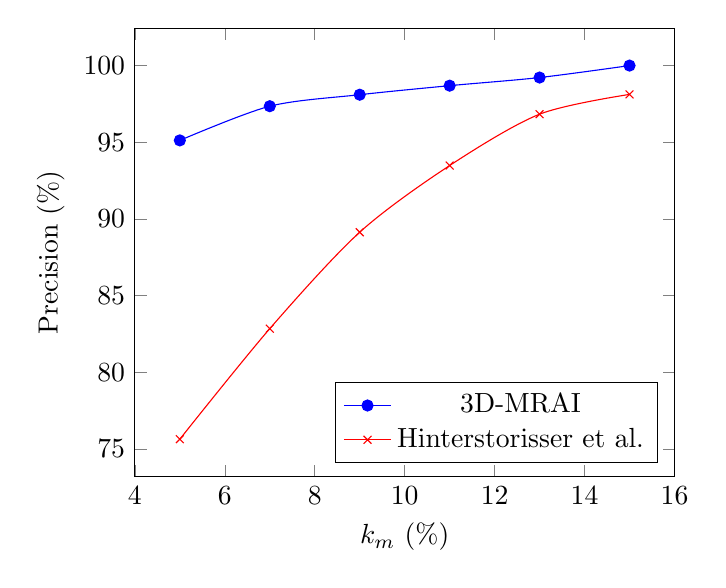
\begin{tikzpicture}
       \begin{axis}[xlabel=$k_m$ (\%),
         ylabel=Precision (\%),
         legend pos=south east,]
         \addplot[smooth, mark=*, blue] plot coordinates {
           (5, 95.12)
           (7, 97.35)
           (9, 98.1)
           (11, 98.69)
           (13, 99.22)
           (15, 100.00)
         };
         \addplot[smooth, mark=x, red] plot coordinates {
           (5, 75.63)
           (7, 82.84)
           (9, 89.13)
           (11, 93.48)
           (13, 96.83)
           (15, 98.12)
         };
         \legend{3D-MRAI,Hinterstorisser et al.}
       \end{axis}
     \end{tikzpicture}
  \caption{3D-MRAI和Hinterstorisser等人的算法准确率曲线}
  \label{fig:mrai}
\end{figure}
表中$k_m$从$5\%$变化到$15\%$,表示物体直径的占比,$k_m$越大,允许的姿态误差就越大,因此准确率就越高。实际实验时,发现$k_m\approx 10\%$时基本上肉眼可以看出匹配的姿态误差。将表\ref{tab:mrai}绘制成图如\ref{fig:mrai}所示,从图中可以发现本文所提出的3D-MRAI算法的准确率大大超过了Hinterstorisser等人的算法,在$k_m=13\%$是3D-MRAI算法的准确率已经接近$100\%$了,以肉眼可以看出匹配的姿态误差$k_m=9\%$为标准时3D-MRAI算法的准确达到了$98.10\%$,比Hinterstorisser等人提出的算法高了大约$9$个百分点。

为了进一步观察算法给出位姿的精度,取$k_m=9\%$时3D-MRAI准确检测的例子,将目标物体的位姿转换为$X,Y,Z,r,p,y$六个直观的变量三维位置和姿态欧拉角,然后于ground truth相比较,得到算法结果在距离和角度上的误差的频率直方图如图\ref{fig:pose-error}所示。
\begin{figure}[ht]
  \centering
  \includegraphics[width=16cm]{pose-error}
  \caption{3D-MRAI算法精度}
  \label{fig:pose-error}
\end{figure}
从图中可以看出3D-MRAI正确检测和估计目标位姿的情况下,在$X,Y,Z$方向下的位置误差大部分分布在$0\sim 1mm$之间,其距离精度在$1mm$左右;在$r,p,y$三个角度下的角度误差也大部分分布在$0\sim 1deg$之间,其角度精度在$1deg$左右。统计图\ref{fig:pose-error}中的数据,可以算出距离误差和角度误差的的均值和方差为:
\begin{equation}
  \begin{array}{ccc}
    e_d &=& 0.82\pm0.21mm\\
    e_a &=& 0.91\pm0.29deg
  \end{array}
\end{equation}

除了关心算法的准确率和精度,算法的运行时间也是我们所关心的。在实验所用的计算机上,本文所设计的3D-MRAI算法与Hinterstorisser等人设计的基于LINEMOD算法的平均帧率如表\ref{tab:mrai-fps}所示。
\begin{table}[ht]
  \centering
  \caption{3D-MRAI和Hinterstorisser等人的算法FPS}
  \begin{tabular}{ccc}
    \toprule
    &Hinterstoisser et al.&\bf{3D-MRAI}\\
    \midrule
    FPS&7.6&2.2\\
    \bottomrule
  \end{tabular}
  \label{tab:mrai-fps}
\end{table}
表中可以看出3D-MRAI的FPS相比Hinterstorisser等人的算法的FPS相对较低,由于使用了深度神经网络相关的算法,涉及到较大的计算量,因此较低的FPS也在情理之中。

综上所述,在$k_m=9\%$时,3D-MRAI算法的准确率为$98.10\%$左右,其估计的位姿的距离精度为$0.82\pm0.21mm$,角度精度为$0.91\pm0.29deg$。

\section{本章小结}
本章介绍了一种基于RGB-D图像的3D目标检测和位姿估计算法3D-MRAI,3D-MARI的核心由检测模块和匹配模块构成。检测模块在Mask R-CNN的基础上通过引入HHA和STN实现在RGB-D图中检测出目标的Mask;匹配模块在4PCS算法的基础上通过点云匹配计算出目标位姿。最后还通过实验与Hinterstorisser等人的算法比较,得出3D-MRAI算法具有更高的检测准确率,并且位姿精度也更高,但在时间性能上略逊于Hinterstorisser等人的算法。

%%% Local Variables:
%%% mode: latex
%%% TeX-master: "../thesis"
%%% End:
